\documentclass{ludis}

% xelatex
\usepackage{fontspec}
\usepackage{xunicode}
\usepackage{xltxtra}

% languages
\usepackage{polyglossia}
\setdefaultlanguage{latvian}
\setotherlanguages{english,russian}
\usepackage{fixlatvian}

% graphics
% \usepackage{pgfplots}
\usepackage{graphicx}
\DeclareGraphicsExtensions{.png,.eps}

% fonts
\setmainfont[Mapping=tex-text]{DejaVu Serif}
\setsansfont[Mapping=tex-text]{DejaVu Sans}
\newfontfamily\russianfont{DejaVu Serif}

% toc
\setcounter{secnumdepth}{3}
\setcounter{tocdepth}{3}

% formatting
% \usepackage{url}
% \usepackage{footnote}
\usepackage{longtable}

% bibtex
\usepackage[pdfauthor={Emīls Šolmanis},%
pdftitle={GPS datu segmentācija},%
pdfkeywords={machine learning, spatial data mining, GPS data analysis, clusterization},%
hidelinks=true,%
pagebackref=false,%
xetex]{hyperref}
\hypersetup{colorlinks=false}
\urlstyle{same}
\usepackage{cite}

\usepackage{xfrac}
%% \usepackage{amsmath}
%% \usepackage{amssymb}
%% \usepackage{enumerate}

\fakultate{Datorikas}
\nosaukums{GPS datu segmentācija}
\darbaveids{Bakalaura}
\autors{Emīls Šolmanis}
\studapl{es09260}
\vaditajs{Asoc. prof., Dr. dat. Jānis Zuters}
\vieta{Rīga}
\gads{2013}

\begin{document}
\maketitle

\begin{abstract-lv}
  Darba mērķis ir izstrādāt neuzraudzītās mašīnmācīšanās algoritmu un atrast pazīmes, kas spētu
  sadalīt ierakstītu GPS datu ceļu atsevišķos fragmentos pēc pārvietošanās metodes bez jebkādas 
  lietotāja atgriezeniskās saites.
  \keywords{mašīnmācīšanās, telpiskā datizrace, GPS datu analīze, \linebreak klasterizācija}
\end{abstract-lv}

\begin{abstract-en}
  The goal of this thesis is to develop an unsupervised machine-learning algo\-rithm and find the 
  necessary features to split a recorded path of GPS coordi\-nates into segments based on
  transportation modes without any explicit user feedback.
  \keywords{machine learning, spatial data mining, GPS data analysis, \linebreak clusterization}
\end{abstract-en}

\tableofcontents

\specnodala{Apzīmējumu saraksts}
\setlength\LTleft{0pt}
\setlength\LTright{0pt}
\begin{longtable}{| c | p{28em} |}
  \hline
  \textbf{Apzīmējums} & \textbf{Atšifrējums}\\ 
  \endhead
  \hline
  GPS & Globālā pozicionēšanas sistēma\\
  \hline
\end{longtable}

\specnodala{Ievads}
GPS ir navigācijas sistēma, kas izmantojot vairākus satelītus nodrošina atbilstoša uztvērēja 
īpašniekam iespēju noteikt savu atrašanās vietu uz Zemes virsmas vai tuvu tai. Mūsdienās
publiski pieejamo sensoru precizitāte ir $\sim 10$ metri. 

Kā jebkuru sensoru rādījumus, arī GPS sensoru rādījumus var ierakstīt, uzglabāt un analizēt. GPS
datus parasti lieto kopā ar informāciju par laiku -- vismaz relatīvo, t.i., sensora iestatīto
iztveršanas intervālu. Tas nepieciešams, lai varētu no datiem iegūt informāciju ne tikai par 
veikto ceļu, bet arī ātrumu.

Šādu datu ievākšanas process ir salīdzinoši vienkāršs, cilvēkam nepieciešams tikai ieslēgt sensoru.
Lielākā problēma plaša mēroga datu ievākšanai ir tas, ka katram sensoram nepieciešams savs 
lietotājs, kā arī, ne mazāk svarīgi, lietotāju privātuma problēmas. Ierakstītie GPS dati dod
precīzu informāciju par lietotāja atrašanās vietu un laiku kamēr vien sensors ir ieslēgts. 
No tiem var izsecināt sensora nēsātāja dzīves vietu, darba vietu, ilgstošākā laika periodā -- 
iespējams arī iepirkšanās vietu preferences un paradumus, hobijus, iemīļotās brīvā laika 
pavadīšanas vietas un laikus.

Iemesli GPS datu vākšanai ir dažādi, taču primāri var izdalīt divas grupas:
\begin{itemize}
\item datu agregēšana, lai iegūtu informāciju par grupas (iespējams, vairāku) uzvedību, piemēram, 
  dažādu ceļu lietojuma intensitāti un laikus, ātri noteikt sastrēgumu vietas, iespējams pat to 
  iemeslus;
\item datu analīze, lai uzlabotu personalizētu informāciju -- piemēram, ceļa plānošanas sistēmas,
  kas spētu pielāgoties konkrēta lietotāja paradumiem un ieteikt tieši šim lietotājam vēlamo ceļu.
\end{itemize}

Klasterizācija ir mašīnmācīšanās / statistikas metode, lai grupētu datu punktus pēc kādas kopīgas
pazīmes.

Darbā gaitā ir izstrādāta metode ierakstītu augstas frekvences GPS ceļu sadalīšanai un 
klasterizācijai pa segmentā izmantotajiem transporta veidiem. Ir pierādīts 
~\cite{zheng_gps_segmentation}, ka ierakstītus GPS ceļus var segmentēt un klasificēt transporta
veidu ar lēmumu kokiem. Klasifikācijas metodes lielākā problēma ir tā, ka iepriekš jāzina 
datos atrodamie transporta veidi, kā arī nepieciešami iezīmēti paraugi, kas pieder katrai grupai.
Šajā darbā izvēlēta klasterizācijas metode, jo tai nav šādu ierobežojumu. Tās galvenā problēma --
iegūtās grupas tiešā veidā nenosaka pārvietošanās veidu vai jebko citu, divu datu punktu esamība
vienā grupā nozīmē tikai to, ka pēc izvēlētās pazīmes tie ir tuvāk viens otram, nekā katrs 
no tiem atsevišķi kādam no citās grupās esošajiem punktiem.

Ir ierakstīti un ievākti iespējami dažādi GPS dati darbā apskatāmās problēmas vajadzībām. 
Darbā izmantotie dati ir ievākti ar \emph{Samsung Galaxy Note (GT-N7000)} viedtālruni, izmantojot
\emph{MyTracks} programmatūru. Datu iztveršanas intervāls tika iestatīts uz mazāko iespējamo,
šajā gadījumā, vienu sekundi. Dati ir ievākti Rīgā, laika periodā no 2012. gada februāra līdz 
2013. gada maijam. Datos ir dati par pārvietošanos ar kājām, braukšanu ar automašīnu, trolejbusu,
autobusu, tramvaju un vilcienu, kā arī braukšanu ar divriteni. Datu pārklājums pilsētas ietvaros 
ir pietiekoši vispārīgs, lai nebūtu pamata domāt par rezultātu novirzi tikai viena konkrēta 
maršruta izvēles dēļ. Attēlā \ref{fig:all_trails} redzamajos ceļos par orientieriem var izmantot
centrā redzamos $4$ tiltus -- no augšas --, Vanšu, Akmens, Salu un Dienvidu.

Apstrādājamo datu formāts ir trijnieki \emph{(garums, platums, laiks)}. Garums un platums doti 
grādos. Tajos nepieciešams atrast pazīmes, kas ļautu noteikt atšķirību starp dažādajiem 
pārvietošanās veidiem. Pamatā, tas nozīmē, ka pieejams ir virziena vektors un laiks -- no tiem
seko arī attālums, ātrums, paātrinājums un virziena maiņa.

\begin{figure}
  \centering
  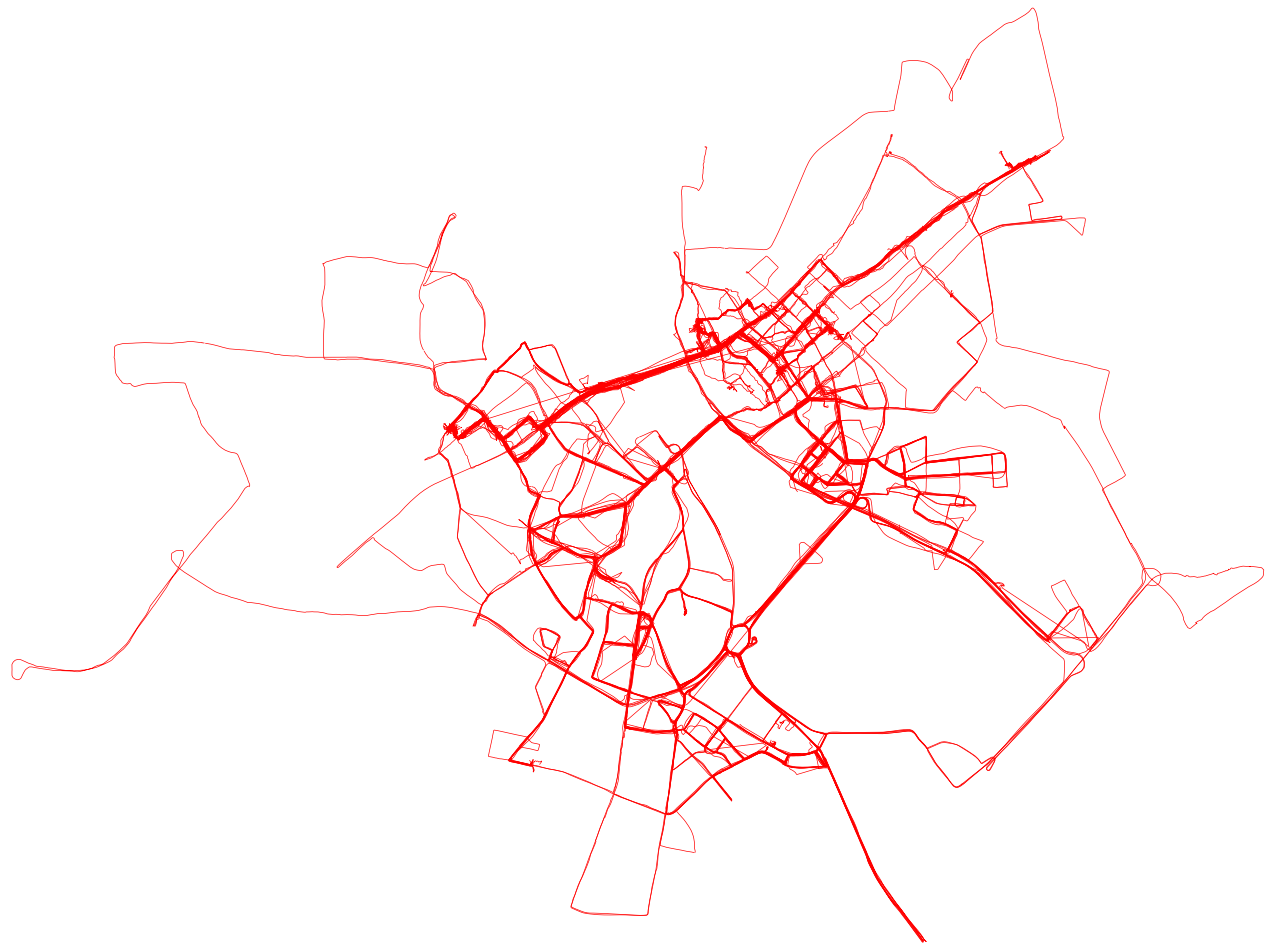
\includegraphics[scale=0.5]{img/all_trails}
  \caption{Ierakstīto datu pārklājums Rīgā}
  \label{fig:all_trails}
\end{figure}

Darbu uzsākot ir izvirzīta hipotēze, ka ir iespējams šos ierakstītos GPS ceļus:
\begin{itemize}
\item sadalīt segmentos pa lietotajām transporta metodēm;
\item veiksmīgi klasterizēt un sagrupēt līdzīgās transporta metodes no dažādiem ierakstītajiem ceļiem.
\end{itemize}

% TODO: darba struktūras apraksts

Darba rezultāti rāda ka ierakstīto ceļu segmentācija un klasterizācija ir iespējama un veiksmīga,
taču nepieciešama tālāka izpēte, lai uzlabotu rezultātu precizitāti.

\chapter{GPS dati}
\section{Datu pieejamība, izplatība}
Mūsdienās ļoti daudzām ierīcēm ir pieejams GPS sensors. Tas ir praktiski jebkurā mūsdienīgā mobilajā
tālrunī un daudzās citās ierīcēs. Piemēram, ASV Federālā Komunikāciju Komisija ir noteikusi, ka līdz
2018. gadam glābšanas dienestu vajadzībām visām bezvadu ierīcēm ir jāspēj būt atrodamām 
ar $50$ pēdu precizitāti ~\cite{fcc_e911}, kas praktiski ir grūti panākams ar torņu triangulācijas 
metodēm un vēl vairāk sekmēs GPS sensoru ieviešanu bezvadu ierīcēs.

Līdz ar GPS ierīču popularitātes un skaita pieaugumu, ir pieaudzis arī šo ierīču ģenerēto datu
plūsmas lielums. Ļoti daudzi lietotāji izmanto GPS sensorus, lai ierakstītu savas sporta aktivitātes,
piemēram, lietotnei Endomondo vien ir $\sim$ $5000000$ - $10000000$ ~\cite{g_play_endomondo} 
lejupielādes Android platformā. \emph{Apple} nepublicē pat aptuvenu statistiku par \emph{iOS}
lejupielādēm.

Ir vairākas lietotnes, kas GPS sniegto informāciju savieno ar sociālajiem tīkliem. Lietotne 
\emph{FourSquare} ļauj lietotājiem ``atzīmēties'' dažādās vietās un par to paziņot lietotnē
apstiprinātajiem draugiem. Dažādas iestādes, piemēram, restorāni, kafejnīcas un bāri, lietotājiem, 
kuri iestādē ``atzīmējušies'' īpaši bieži, sniedz atlaides saviem pakalpojumiem. Līdzīgi,
Google lietotne \emph{Latitude} sniedz iespēju apstiprinātiem draugiem reālā laikā redzēt
lietotāja viedtālruņa atrašanās vietu.

Ir pieejamas arī lietotnes, kas mēģina sekot un kategorizēt lietotāju ikdienas 
aktivitātes, kā piemēram \emph{iOS} pieejamā lietotne \emph{Moves} ~\cite{moves_app}, taču tā 
izmanto telefona akselerometru, žiroskopu un GPS sensoru, kas:
\begin{itemize}
\item negatīvi iespaido baterijas darbības ilgumu;
\item padara lietotnes izmantošanu neiespējamu uz ierīcēm, kas aprīkotas tikai ar GPS sensoru.
\end{itemize}

GPS dati tiek plaši lietoti arī paplašinātās realitātes produktos. Arī nesen izlaistajā paplašinātās
realitātes briļļu produktā \emph{Google Glass} ir GPS sensors, un tas palīdz daudzām lietotnēm
noteikt pareizo kontekstu un sniegt lietotājam labākas rekomendācijas. Piemēram, redzot tikai bildi
ar Eifeļa torni mēs nevaram pateikt, vai skatamies uz Eifeļa torni Parīzē vai kādu mazāku repliku
Las Vegasā. GPS informācija daļēji ir integrēta Google produktos jau šobrīd, meklējot kartes
lietotnēs ``kafejnīca'' tiks atrastas tuvākās pieejamās kafejnīcas u. tml.

Visu šo apstākļu rezultātā, pieejamo GPS datu plūsma ir iespaidīgi piaugusi, un tā turpina augt.
Taču šos datus ir jāanalizē, no tiem jāizgūst derīga informācija, jo GPS dati paši par sevi ir
tikai laika un vietas pāris.

\section{Mašīnmācīšanās metodes}
Mašīnmācīšanās mākslīgā intelekta apakšnozare, kas balstoties uz empīriskiem datiem un novērojumiem
izveido tiem atbilstošu uzvedības modeli. 

Tā kā mašīnmācīšanās nozare izmanto uz empīriskus datus, lielākā daļa mašīnmācīšanās
algoritmu metožu ir balstītas statistikā un varbūtību teorijā. 

Parasti izšķir uzraudzīto un neuzraudzīto mašīnmācīšanos. Uzraudzītā mašīnmācīšanās tiek lietota
tad, kad ir zināms, kāds rezultāts ir ``pareizs'' un ir pieejami pareizo rezultātu paraugi.
Modelis tiek veidots tā, lai imitētu esošos ``pareizos'' datu paraugus un vēlāk testēts uz 
apmācības procesā neizmantotiem datiem. Neuzraudzītā mašīnmācīšanās tiek lietota gadījumos, kad
nav pieejama informācija par to, kurš datu paraugs ir ``pareizs''. To lieto lai atrastu datos
apslēptas struktūras. Viena no plašākajām neuzraudzītās mašīnmācīšanās nozarēm ir klasterizācija.

Klasterizācija ir neuzraudzītās mašīnmācīšanās metode, kuras mērķis ir grupēt pieejamos datu
paraugus pēc kādas kopīgas pazīmes tā, lai paraugi, kas atrodas vienā grupā būtu tuvāk viens otram,
nekā tie ir paraugiem no citām grupām. 

\chapter{Uzdevuma izpēte}
\section{Problēmas būtība, motivācija}
Darba ietvaros tiek izstrādāta metode, kā sadalīt ierakstītus GPS ceļus atsevišķos segmentos
pēc transporta veida un šos segmentus apkopotu grupās tā, ka grupas ietvaros segmentiem ir viens
transporta veids.

Šāda algoritma pieejamība nozīmētu to, ka cilvēkiem nevajadzētu datus iezīmēt. Rastos iespēja
izmantot, piemēram, anonīmi ziedotus datus. Cilvēki varētu ierakstīt savu pārvietošanos
un nodot apstrādei automatizētai sistēmai.

Ar šādu algoritmu iegūstot konkrēta lietotāja izmantotos transportus kādos ceļu posmos varētu veidot
personalizētas ceļu plānošanas sistēmas. Piemēram, ja lietotājs konkrētos ceļa posmos parasti
dod priekšroku braukšanai ar divriteni, nevis sabiedrisko transportu, tad meklējot ceļu uz galamērķi,
uz kuru tuvākais ceļš ievērojami pārklājas ar šiem ceļa posmiem, primārā rekomendācija būtu
braukt ar divriteni.

Ja būtu pieejami pietiekoši daudz dati, šos segmentus varētu izmantot pilsētas infrastruktūras
optimizācijai. Piemēram, būtu redzams, kurās vietās pa ietvi intensīvi pārvietojas velobraucēji,
un attiecīgi prioretizēt veloceliņu izbūvi koncentrējoties uz šīm vietām. Tāpat būtu redzams cik
intensīvi kādos posmos cilvēki lieto sabiedrisko transportu -- iespējams, ka viena maršruta ietvaros
intensīvi izmantots tiek tikai kāds konkrēts posms.

\section{Pastāvošie risinājumi}
Līdz šim nav izstrādāts algoritms un tā implementācija, kas ļautu segmentēt GPS ierakstu daļās un 
šīs daļas veiksmīgi grupēt bez lietotāja atgriezeniskās saites un papildus informācijas ievada
sistēmā (piemēram, sabiedriskā transporta maršrutiem un sarakstiem).

Visvairāk darba šajā jomā pēdējo gadu laikā veikuši \emph{Microsoft Research Asia} projekta
\emph{GeoLife} ietvaros. Šī projekta ietvaros ir izstrādāts uzraudzītās mašīnmācīšanās 
algoritms, kas balstās uz lēmumu kokiem. ~\cite{zheng_gps_segmentation} Šajā \emph{Microsoft Research}
darbā ņemti vērā arī svarīgākie pirms tam veiktie atklājumi, taču šis ir pirmais nopietnais
darbs, kas apskata transporta veidu izgūšanas problēmu.

Kaut arī minētajam algoritmam ir salīdzinoši augsta precizitāte, tā lielākie trūkumi ir saistīti
ar to, ka tas ir uzraudzītās mašīnmācīšanās algoritms. Tas nozīmē laikietilpīgu un apjomīgu datu
ievākšanas procesu. Kādam -- parasti pašiem datu autoriem -- ir jāiezīmē dati. Šādus iezīmētus
datus ir jāievāc pietiekoši daudz un vēlams arī apmēram vienmērīgā daudzumā pa dažādajām klasēm,
lai algoritms spētu veiksmīgi apmācīties. Turklāt pat šādā gadījumā, algoritmam ir mērogošanas
problēmas -- tas pēc definīcijas spēs atpazīt tikai tos transporta veidus, uz kuriem būs
apmācīts. \emph{Microsoft Research} darba ietvaros ir minēta klasifikācija starp staigāšanu,
braukšanu ar automašīnu, braukšanu ar sabiedrisko transportu un braukšanu ar velosipēdu. Šie
transporta veidi ir raksta autoru izvēlēti. Brīdī, kad reālajos datos parādās citi transporta
veidi
\begin{itemize}
\item labākajā gadījumā algoritma autori to pamana -- tad ir jāievāc dati par jauno transporta
  veidu un no jauna jāapmāca algoritms;
\item sliktākajā gadījumā -- neviens nepamana, ka datos parādījies jauns transporta veids un šis
  jaunais transporta veids tiek konsekventi nepareizi klasificēts kā viens no zināmajiem.
\end{itemize}

\chapter{Iespējamie problēmas risinājumi}
GeoLife projekta ietvaros izstrādātajam algoritmam GPS ceļu segmentācijai ir priekšrocības 
pār alternatīvajām ``vienmērīgā laika'' un ``vienmērīgā attāluma'' metodēm, un tās ir
eksperimentāli demonstrētas -- reālajā dzīvē cilvēku pārvietošanās veidu sadalījums laikā 
un attālumā nav ne tuvu vienmērīgs, tādēļ izstrādātais maiņas-punktu algoritms strādā labāk.
Algoritma veiktspēja ir pietiekoša -- tipiski $\sim$ $35\%$ - $40\%$
precizitāte un $\sim$ $70\%$ - $80\%$ jutība ~\cite{zheng_gps_segmentation} -- 
lai neuzskatītu to par primāro problēmu, izmantotu tā implementāciju GPS ceļu segmentēšanai 
un pievērstos atrasto segmentu grupēšanas problēmai un, kad tiks atrasts piemērots risinājums
segmentu grupēšanai, atgrieztos pie šīs daļas precizitātes uzlabošanas.

Līdzīgu segmentu grupēšana pēc kādām pazīmēm ir klasifikācijas vai klasterizācijas problēma. Tā kā
darba mērķis ir izslēgt jebkādu atgriezenisku saiti ar lietotāju, un klasifikācija ir uzraudzītās
mašīnmācīšanās problēma, risinājumi jebkurā gadījumā būs saistīti ar klasterizāciju.

\chapter{Problēmas risinājums}
\section{Pieejas izklāsts}
Darbā apskatāmajai problēmai ir divi posmi:
\begin{enumerate}
\item sadalīt ierakstītos GPS ceļus segmentos ar dažādiem transporta veidiem;
\item sagrupēt iegūtos segmentus pa transporta veidiem.
\end{enumerate}

Sākotnējā izpēte norāda uz to, ka pirmo posmu var risināt izmantojot maiņas-punktu algoritmu 
~\cite{zheng_gps_segmentation}, jo tā veiktspēja ir pietiekoši augsta.

Lai risinātu problēmas otro posmu, nepieciešams veids, kā grupēt dažādos iegūtos segmentus.
Šajā darbā tā tiek apskatīta kā klasterizācijas problēma. Taču pirms varam nodarboties ar 
datu klasterizāciju, nepieciešamas pazīmes pēc kurām šos datus klasterizēt.

\section{Pazīmju analīze}
\subsection{Ātrums}
Attēlā \ref{fig:speed_comparison} redzams dažādu transporta līdzekļu pārvietošanās ātrumu grafisks
salīdzinājums. Pārskatāmības labad grafiki nolīdzināti ar $(3, 5)$ modificēto Daniell filtru.

Modificētais Daniell filtrs ~\cite{daniell1946} ar platumu $m$ tiek definēts kā 
\begin{align*}
  w_i = \begin{cases}
    \frac{1}{2 (m - 1)} &\text{, ja i = 1 vai i = m}\\
    \frac{1}{m - 1} &\text{ citādi}
    \end{cases}
\end{align*}
Notācija $(3, 5)$ nozīmē secīgu filtru ar platumu $3$ un $5$ pielietošanu, kas ir vienlīdzīga
abu filtru konvolūcijas pielietošanai.

% par(family="AvantGarde")
% k <- kernel("modified.daniell", c(3, 5));
% plot(kernapply(andrejsala$speed[walk], k), type="l", ylim=c(0, 25), xlim=c(0, 900), col="green", lty="dashed", main="Pārvietošanās ātrumi", xlab="Laiks (s)", ylab="Ātrums (m/s)")
% lines(kernapply(andrejsala$speed[drive1], k), type="l", col="red", lty="dotted")
% lines(kernapply(andrejsala$speed[drive2], k), type="l", col="red", lty="dotted")
% lines(kernapply(andrejsala$speed[bike], k), type="l", col="blue", lty="longdash")
% lines(kernapply(homeUni$speed[trolley], k), type="l", col="black", lty="twodash")
% legend(0, 23, c("Iešana", "Auto", "Divritens", "Trolejbuss"), col=c("green", "red", "blue", "black"), lty=c("dashed", "dotted", "longdash", "twodash"))
\begin{figure}
  \centering
  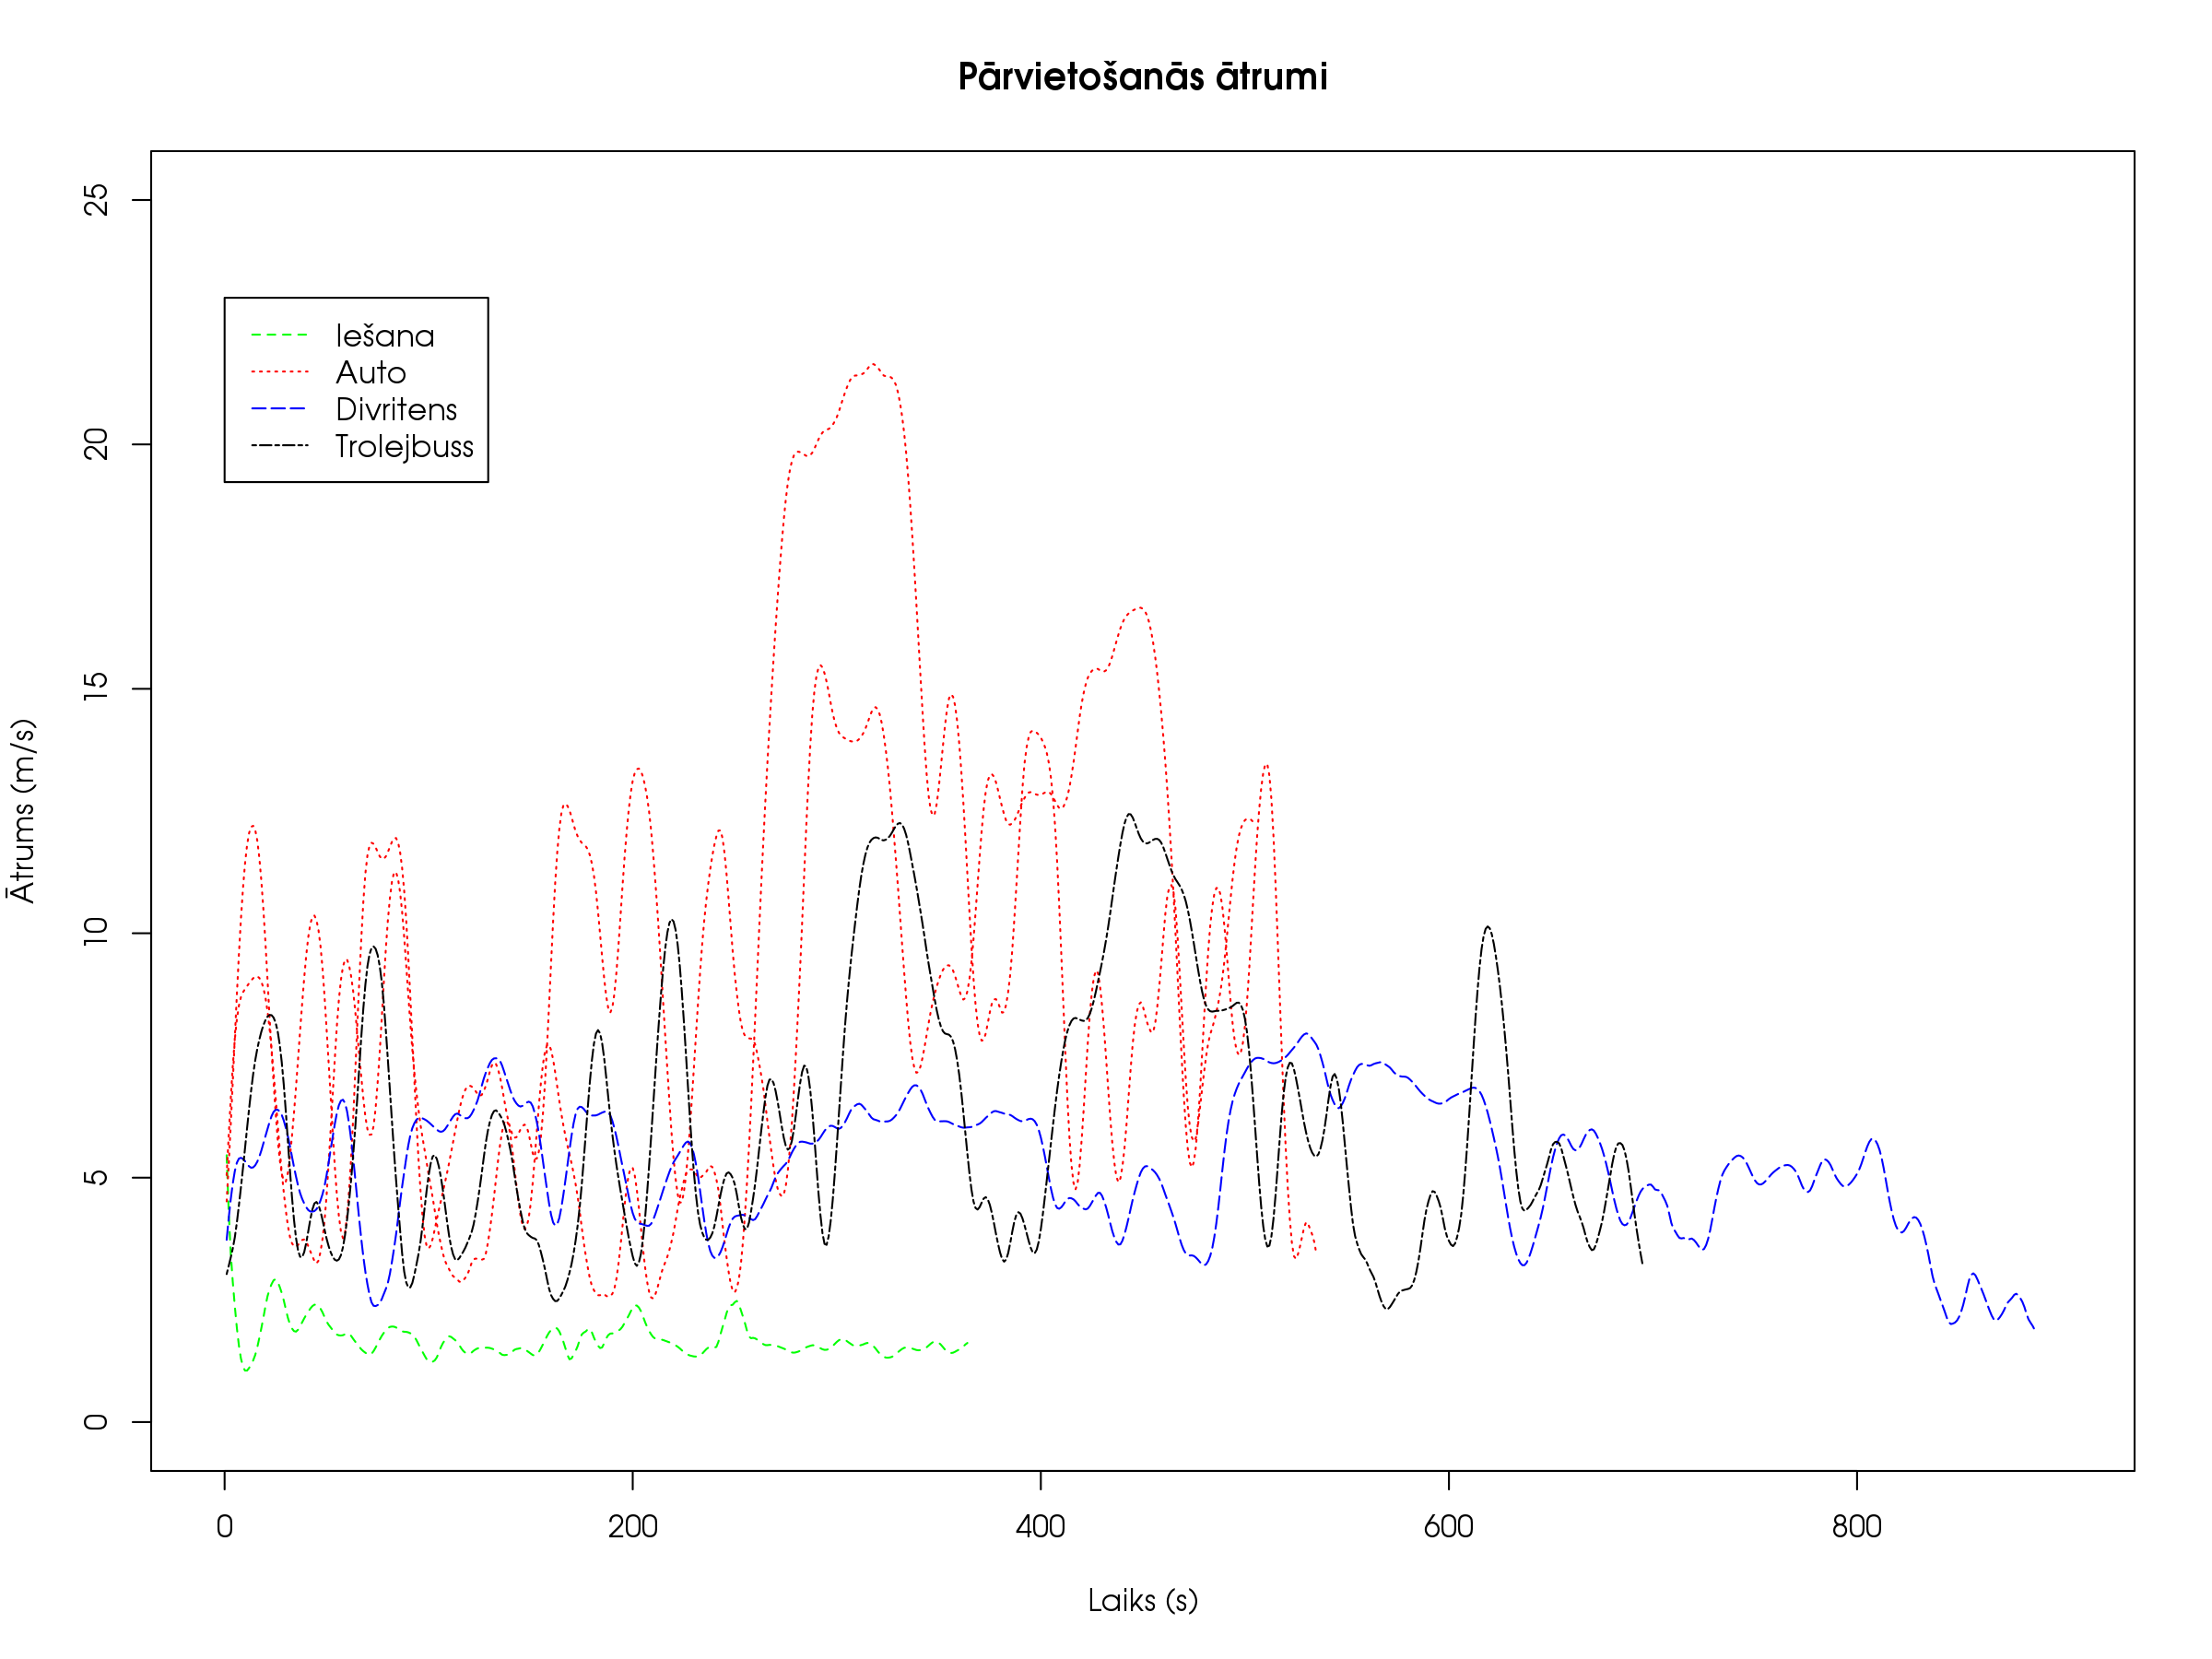
\includegraphics[scale=0.5]{img/speed_comparison}
  \caption{Dažādu transportu pārvietošanās ātrumu salīdzinājums}
  \label{fig:speed_comparison}
\end{figure}

Kā redzams attēlā, dotajā gadījumā cilvēkam ir iespējams salīdzinoši skaidri nošķirt transporta 
veidus jau pēc ātrumiem, taču tikai tad, ja novērojumi veikti pietiekoši ilgā laika periodā.
Attēlā redzams, ka apmēram pirmās $250$ - $300$ sekundes braukšanu ar trolejbusu, auto un divriteni
ir grūti atšķirt. Zinot lietotos transporta veidus un, galvenokārt, to, ka jāmeklē tieši $4$ 
atšķirīgi, tos ir iespējams izšķirt, taču šādas zināšanas eksperimenta ietvaros nav dotas.

Attēlā \ref{fig:speed_comparison} redzams arī tas, ka jau tikai pēc ātruma ir viegli nošķirt iešanu
ar kājām no pārējiem pārvietošanās veidiem, kas apstiprina \emph{GeoLife} projekta ietvaros
izstrādāto metodi no sākuma grupēt segmentus grupās ``staigāšana'' un ``ne-staigāšana'' un tikai
pēc tam klasificēt segmentus, kas ir ``ne-staigāšana'' grupā. ~\cite{zheng_gps_segmentation}

% par(family="AvantGarde")
% k <- kernel("modified.daniell", c(3, 5))
% plot(kernapply(andrejsalaAccels$acceleration[walk], k), type="l", ylim=c(-1.0, 1.0), xlim=c(0, 300), lty="dashed", col="green", main="Pārvietošanās paātrinājumi", xlab="Laiks (s)", ylab="Paātrinājums (m/s²)")
% lines(kernapply(andrejsalaAccels$acceleration[drive1], k), type="l", lty="dotted", col="red")
% lines(kernapply(andrejsalaAccels$acceleration[bike], k), type="l", lty="longdash", col="blue")
% lines(kernapply(homeUniAccels$acceleration[trolley], k), type="l", lty="twodash", col="black")
% legend(20, 1.0, c("Iešana", "Auto", "Divritens", "Trolejbuss"), col=c("green", "red", "blue", "black"), lty=c("dashed", "dotted", "longdash", "twodash"))
\subsection{Paātrinājums}
Attēlā \ref{fig:acceleration_comparison} redzams dažādu pārvietošanās veidu paātrinājumu 
salīdzinājums. Pārskatāmības labad grafiki nolīdzināti ar $(3, 5)$ modificēto Daniell filtru.

\begin{figure}
  \centering
  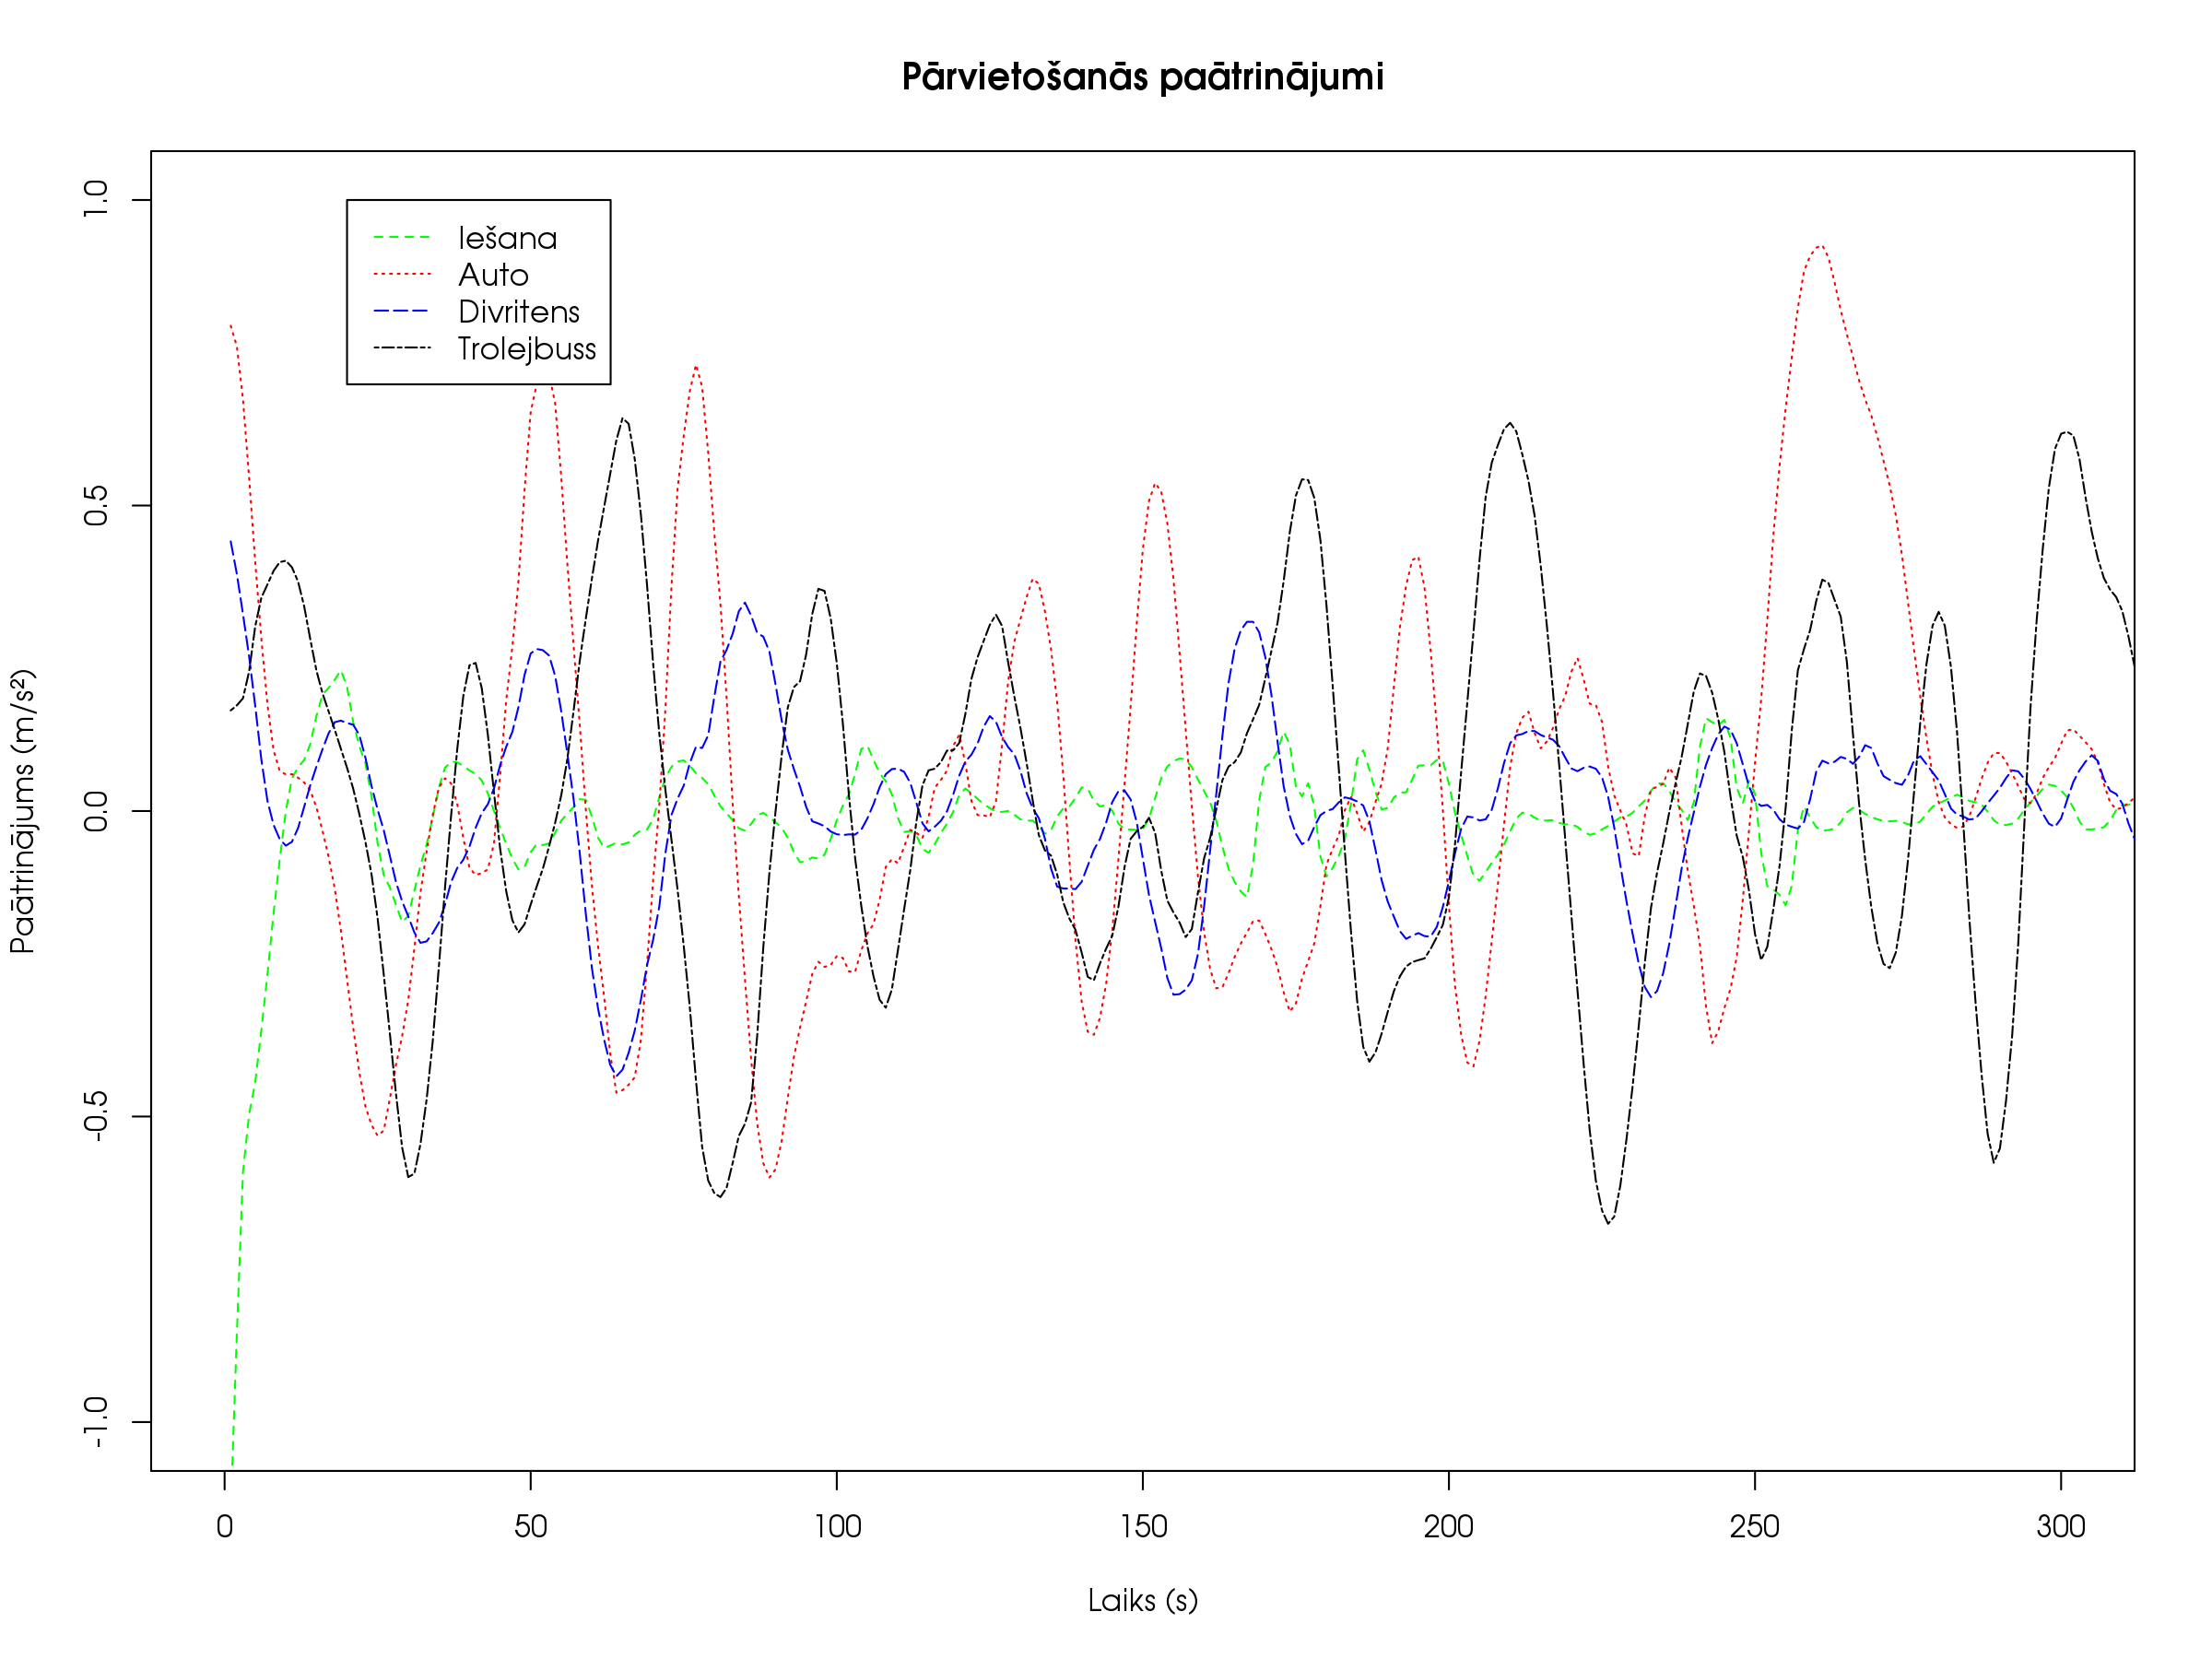
\includegraphics[scale=0.5]{img/acceleration_comparison}
  \caption{Dažādu transportu pārvietošanās paātrinājumu salīdzinājums}
  \label{fig:acceleration_comparison}
\end{figure}

Arī pēc paātrinājuma visvieglāk ir atšķirt iešanu ar kājām no pārējiem pārvietošanās veidiem. 
Amplitūdu atšķirības nav pārāk lielas absolūto vērtību ziņā, taču relatīvi tās ir vērā ņemamas.

Piemēram, redzams, ka, braucot ar divriteni, paātrinājuma amplitūda ir $0.44\,\sfrac{m}{s^2}$,
braucot ar auto -- $0.92\,\sfrac{m}{s^2}$, braucot ar trolejbusu -- $0.65\,\sfrac{m}{s^2}$, 
bet ejot ar kājām -- $0.23\,\sfrac{m}{s^2}$ \emph{(vērtības nogludinātajai līknei)}. 

Tātad pārvietojoties ar divriteni paātrinājuma amplitūda ir $2$ reizes
lielāka, nekā pārvietojoties ar kājām, un pārvietojoties ar auto tā ir $2$ reizes lielāka nekā
braucot ar divriteni. Paātrinājuma amplitūda pārvietojoties ar trolejbusu ir pa vidu starp
divriteņa un auto rādītājiem un bez lielas noslieces uz kādu no tiem. Tas, savukārt, liek domāt,
ka paātrinājums varētu būt ļoti labs rādītājs, lai izšķirtu dažādos pārvietošanās veidus -- jau
pēc amplitūdām vien mēs varam diezgan viennozīmīgi izšķirt šos četrus transportus.

Taču amplitūdas nav vienīgais svarīgais rādītājs, kas redzams šajā attēlā. Ir skaidri redzamas
atšķirības attēloto paātrinājumu frekvencēs. Iešanas paātrinājums mainās visātrāk, auto
un trolejbusam tas ir līdzīgs, taču auto paātrinājumam šķietami ir arī ātrāk mainīgas komponentes
un trolejbusa paātrinājums ir vienmērīgāks. Pārvietojoties ar divriteni, paātrinājums mainās
vislēnāk.

Tas liek domāt, ka būtu lietderīgi veikt padziļinātu frekvenču analīzi paātrinājumiem.

% par(mfrow=c(2, 2),
%     family="AvantGarde",
%     oma=c(0, 0, 2, 0),
%     mai=c(0.1, 0.4, 0.4, 0.1)); # bottom left top right
% fftData <- andrejsalaAccels$acceleration[walk]; 
% barplot(Mod(fft(fftData) / length(fftData)), main="Iešana");
% fftData <- andrejsalaAccels$acceleration[drive1]; 
% barplot(Mod(fft(fftData) / length(fftData)), main="Automašīna");
% fftData <- andrejsalaAccels$acceleration[bike]; 
% barplot(Mod(fft(fftData) / length(fftData)), main="Divritenis");
% fftData <- homeUniAccels$acceleration[trolley]; 
% barplot(Mod(fft(fftData) / length(fftData)), main="Trolejbuss");
% title(main="Nenolīdzinātu paātrinājumu Furjē analīze", outer=TRUE, cex.main=2);

\begin{figure}
  \centering
  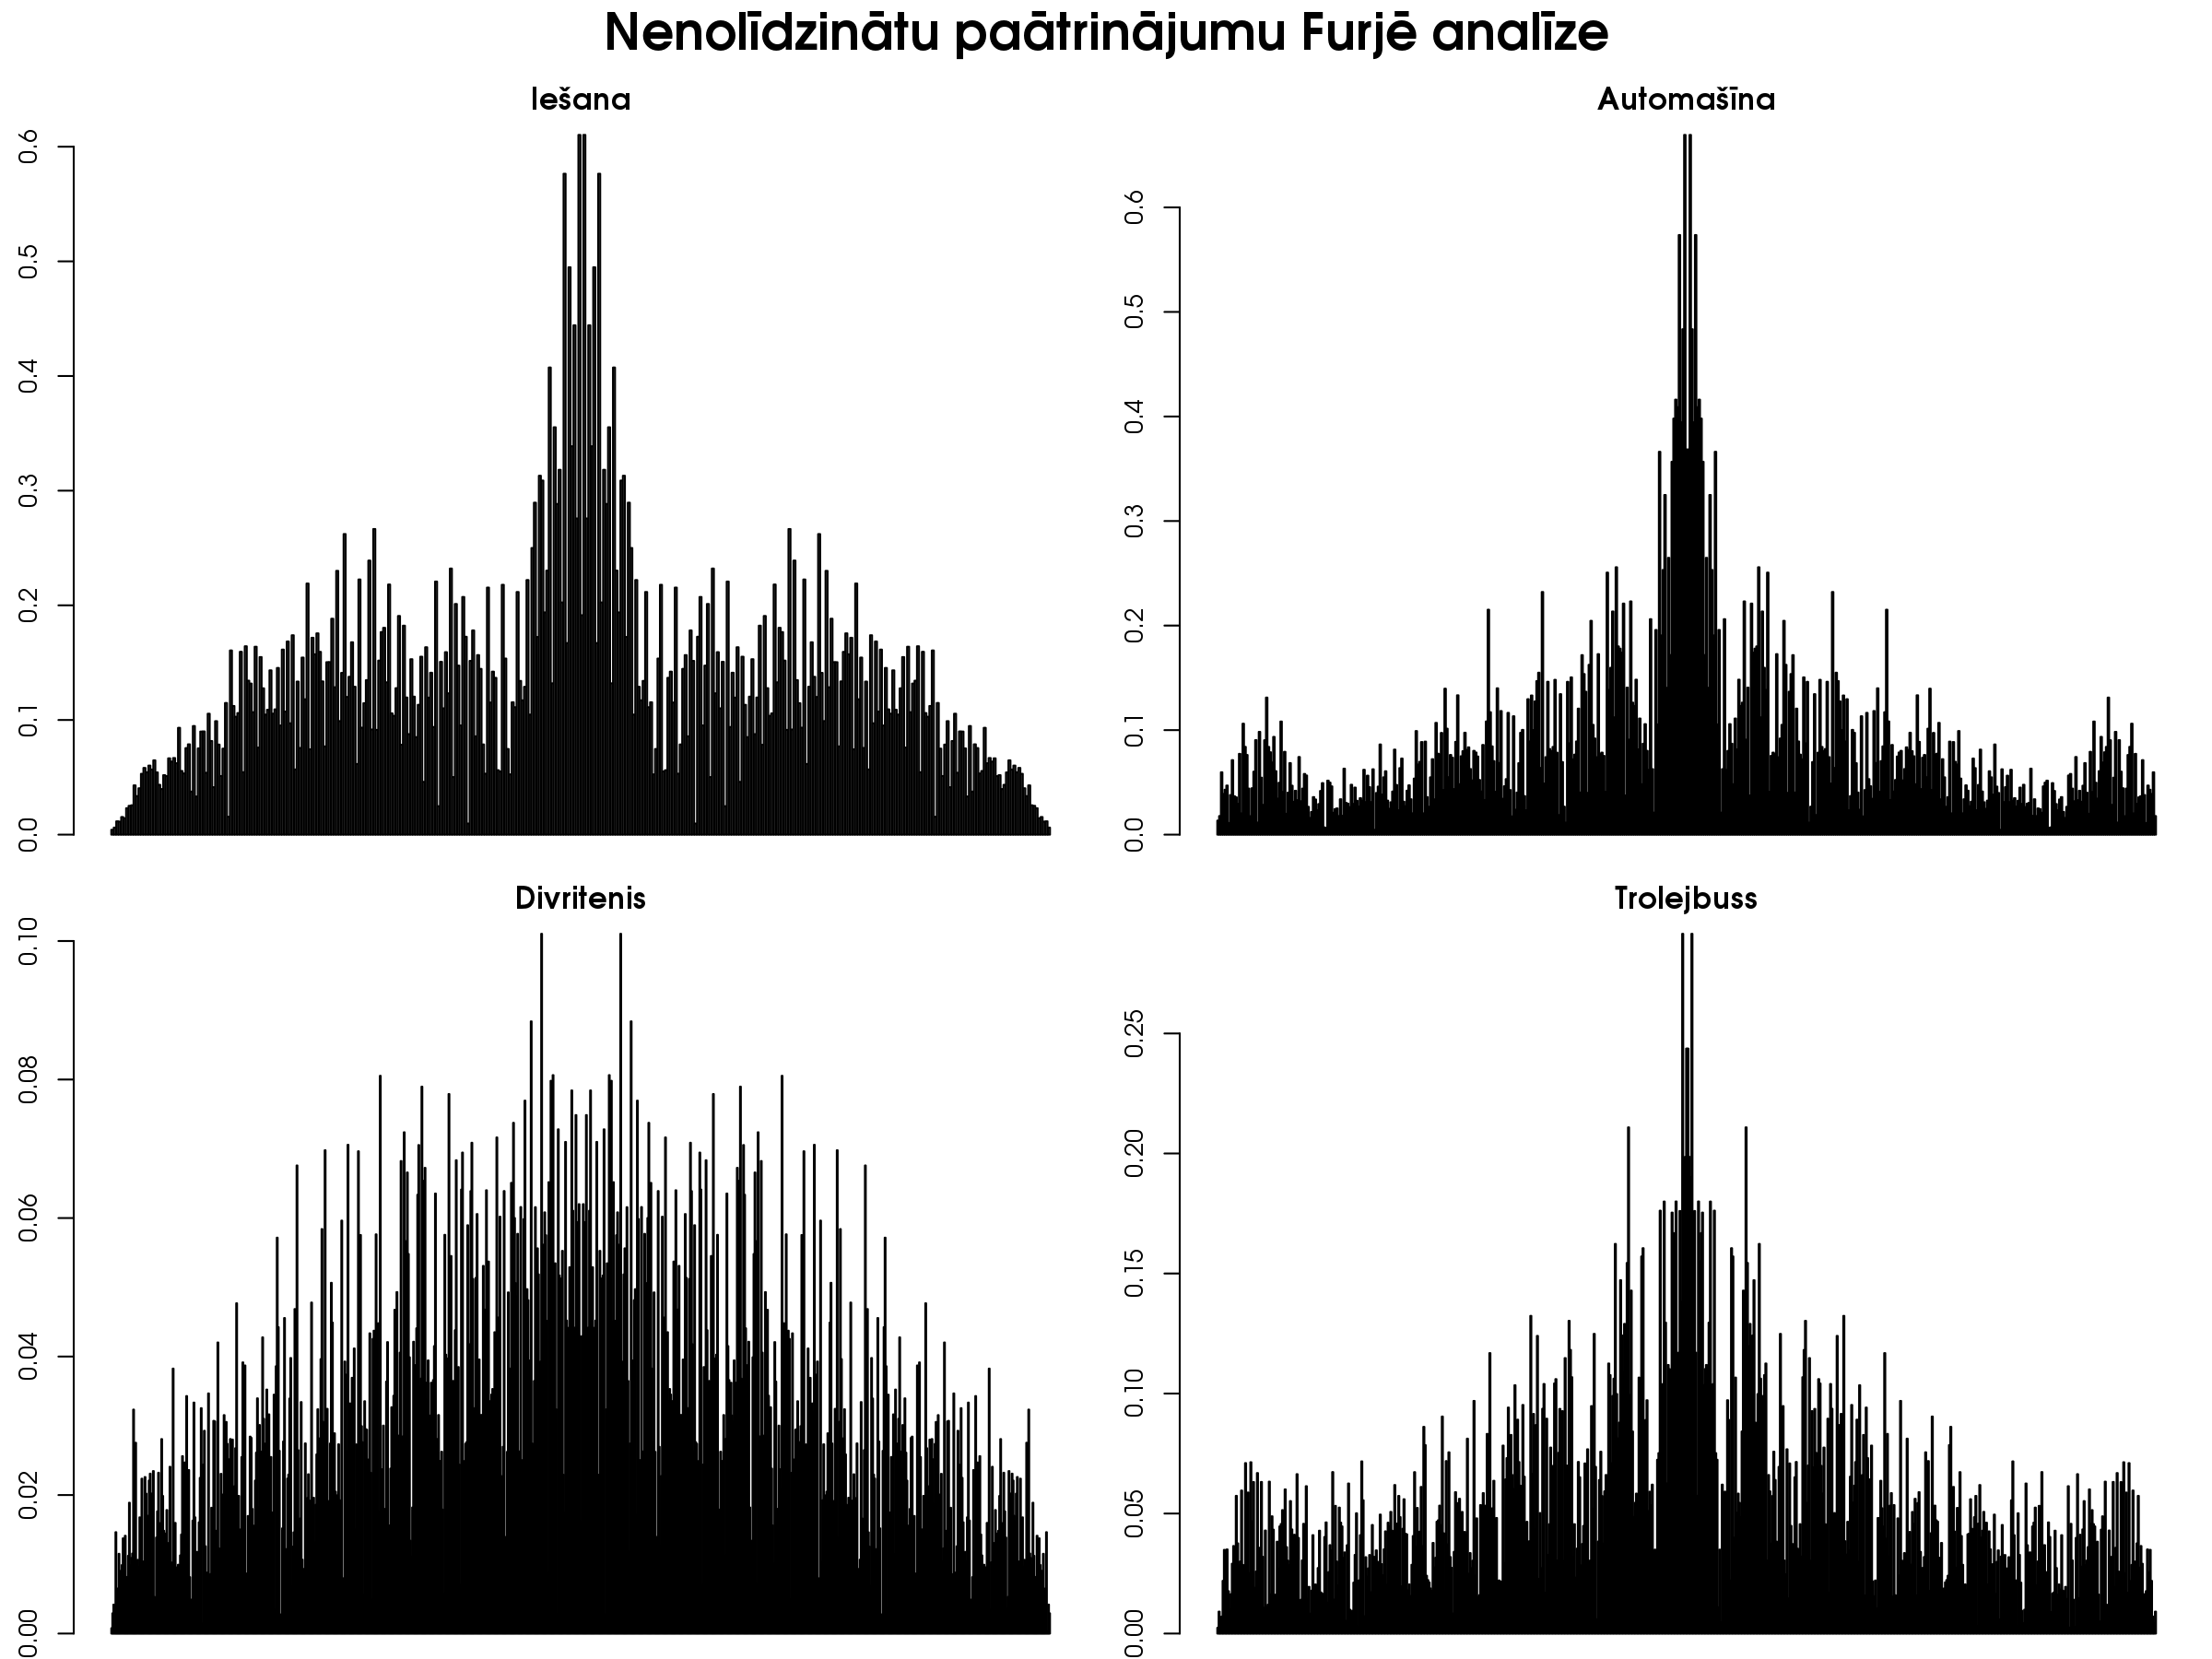
\includegraphics[scale=0.5]{img/fourier_analysis}
  \caption{Dažādu transportu pārvietošanās paātrinājumu Furjē analīze}
  \label{fig:fourier_analysis}
\end{figure}

Lai noteiktu signāla frekvenču komponentes, lieto Furjē transformāciju. Diskrētā Furjē transformācija
tiek definēta kā 
\begin{align*}
  \omega &= \exp \left (\frac{2 \pi i}{N} \right)\\
  x_k &= \sum_{n = 0}^{N - 1} x_n \cdot \omega^{-kn}
\end{align*}
un tā transformē signālu no laika vērtību apgabala uz frekvenču vērtību apgabalu.

Paātrinājumu Furjē komponenšu absolūtās vērtības attēlotas 
grafikā \ref{fig:fourier_analysis}. Redzams, ka tās manāmi atšķiras transporta veidiem. Iešanai ar
kājām ir izteiktas augstās frekvences komponentes un salīdzinoši spēcīgas arī vidējās frekvences.
Paātrinājumam braucot ar auto spēcīgās frekvences ir daudz koncentrētākas tieši augstajās.
Braukšanai ar divriteni ir mazākas amplitūdas un vienmērīgāk pārstāvēts spektrs, savukārt trolejbusa
paātrinājumam ir divi izteikti ``pīķi'' augstajā frekvenču zonā un vidējas amplitūdas.

Furjē analīze tālāk apstiprina hipotēzi par paātrinājumu kā piemērotu pazīmi segmentu 
klasterizācijai. 

\section{Klasterizācija}
Furjē transformācijas rezultāts ir kompleksu skaitļu kopa, kas izsaka laika virknes datus
kā vairāku, dažādu frekvenču, sinusoīdu summu un norāda šo sinusoīdu amplitūdas un fāzes nobīdes.
Šie dati acīmredzami tiešā veidā nav piemēroti klasterizācijas problēmas risināšanai, jo:
\begin{itemize}
\item transformācijas rezultāts ir simetrisks; pastāv informācijas dubultošanās;
\item transformācijas rezultāts ir komplekss.
\end{itemize}

Lai risinātu klasterizācijas problēmu, mums nepieciešama metrika, kas izsaka tieši cik lielu 
ietekmi uz visu signālu izdara katra periodiskā komponente. To var veiksmīgāk panākt ar 
spektrālo analīzi un periodogrammām. ~\cite{bloomfield2004} Periodogrammu definē kā
\begin{align*}
  I(f) = n | d(f) |^2
\end{align*}
kur $d(f)$ ir diskrētā Furjē transformācija.

Transporta veidu paātrinājumu periodogrammas attēlotas attēlā \ref{fig:periodograms}. Pielietota
nolīdzināšana ar modificēto Daniell filtru $(5, 9)$, lai mazinātu mērījuma trokšņus.

\begin{figure}
  \centering
  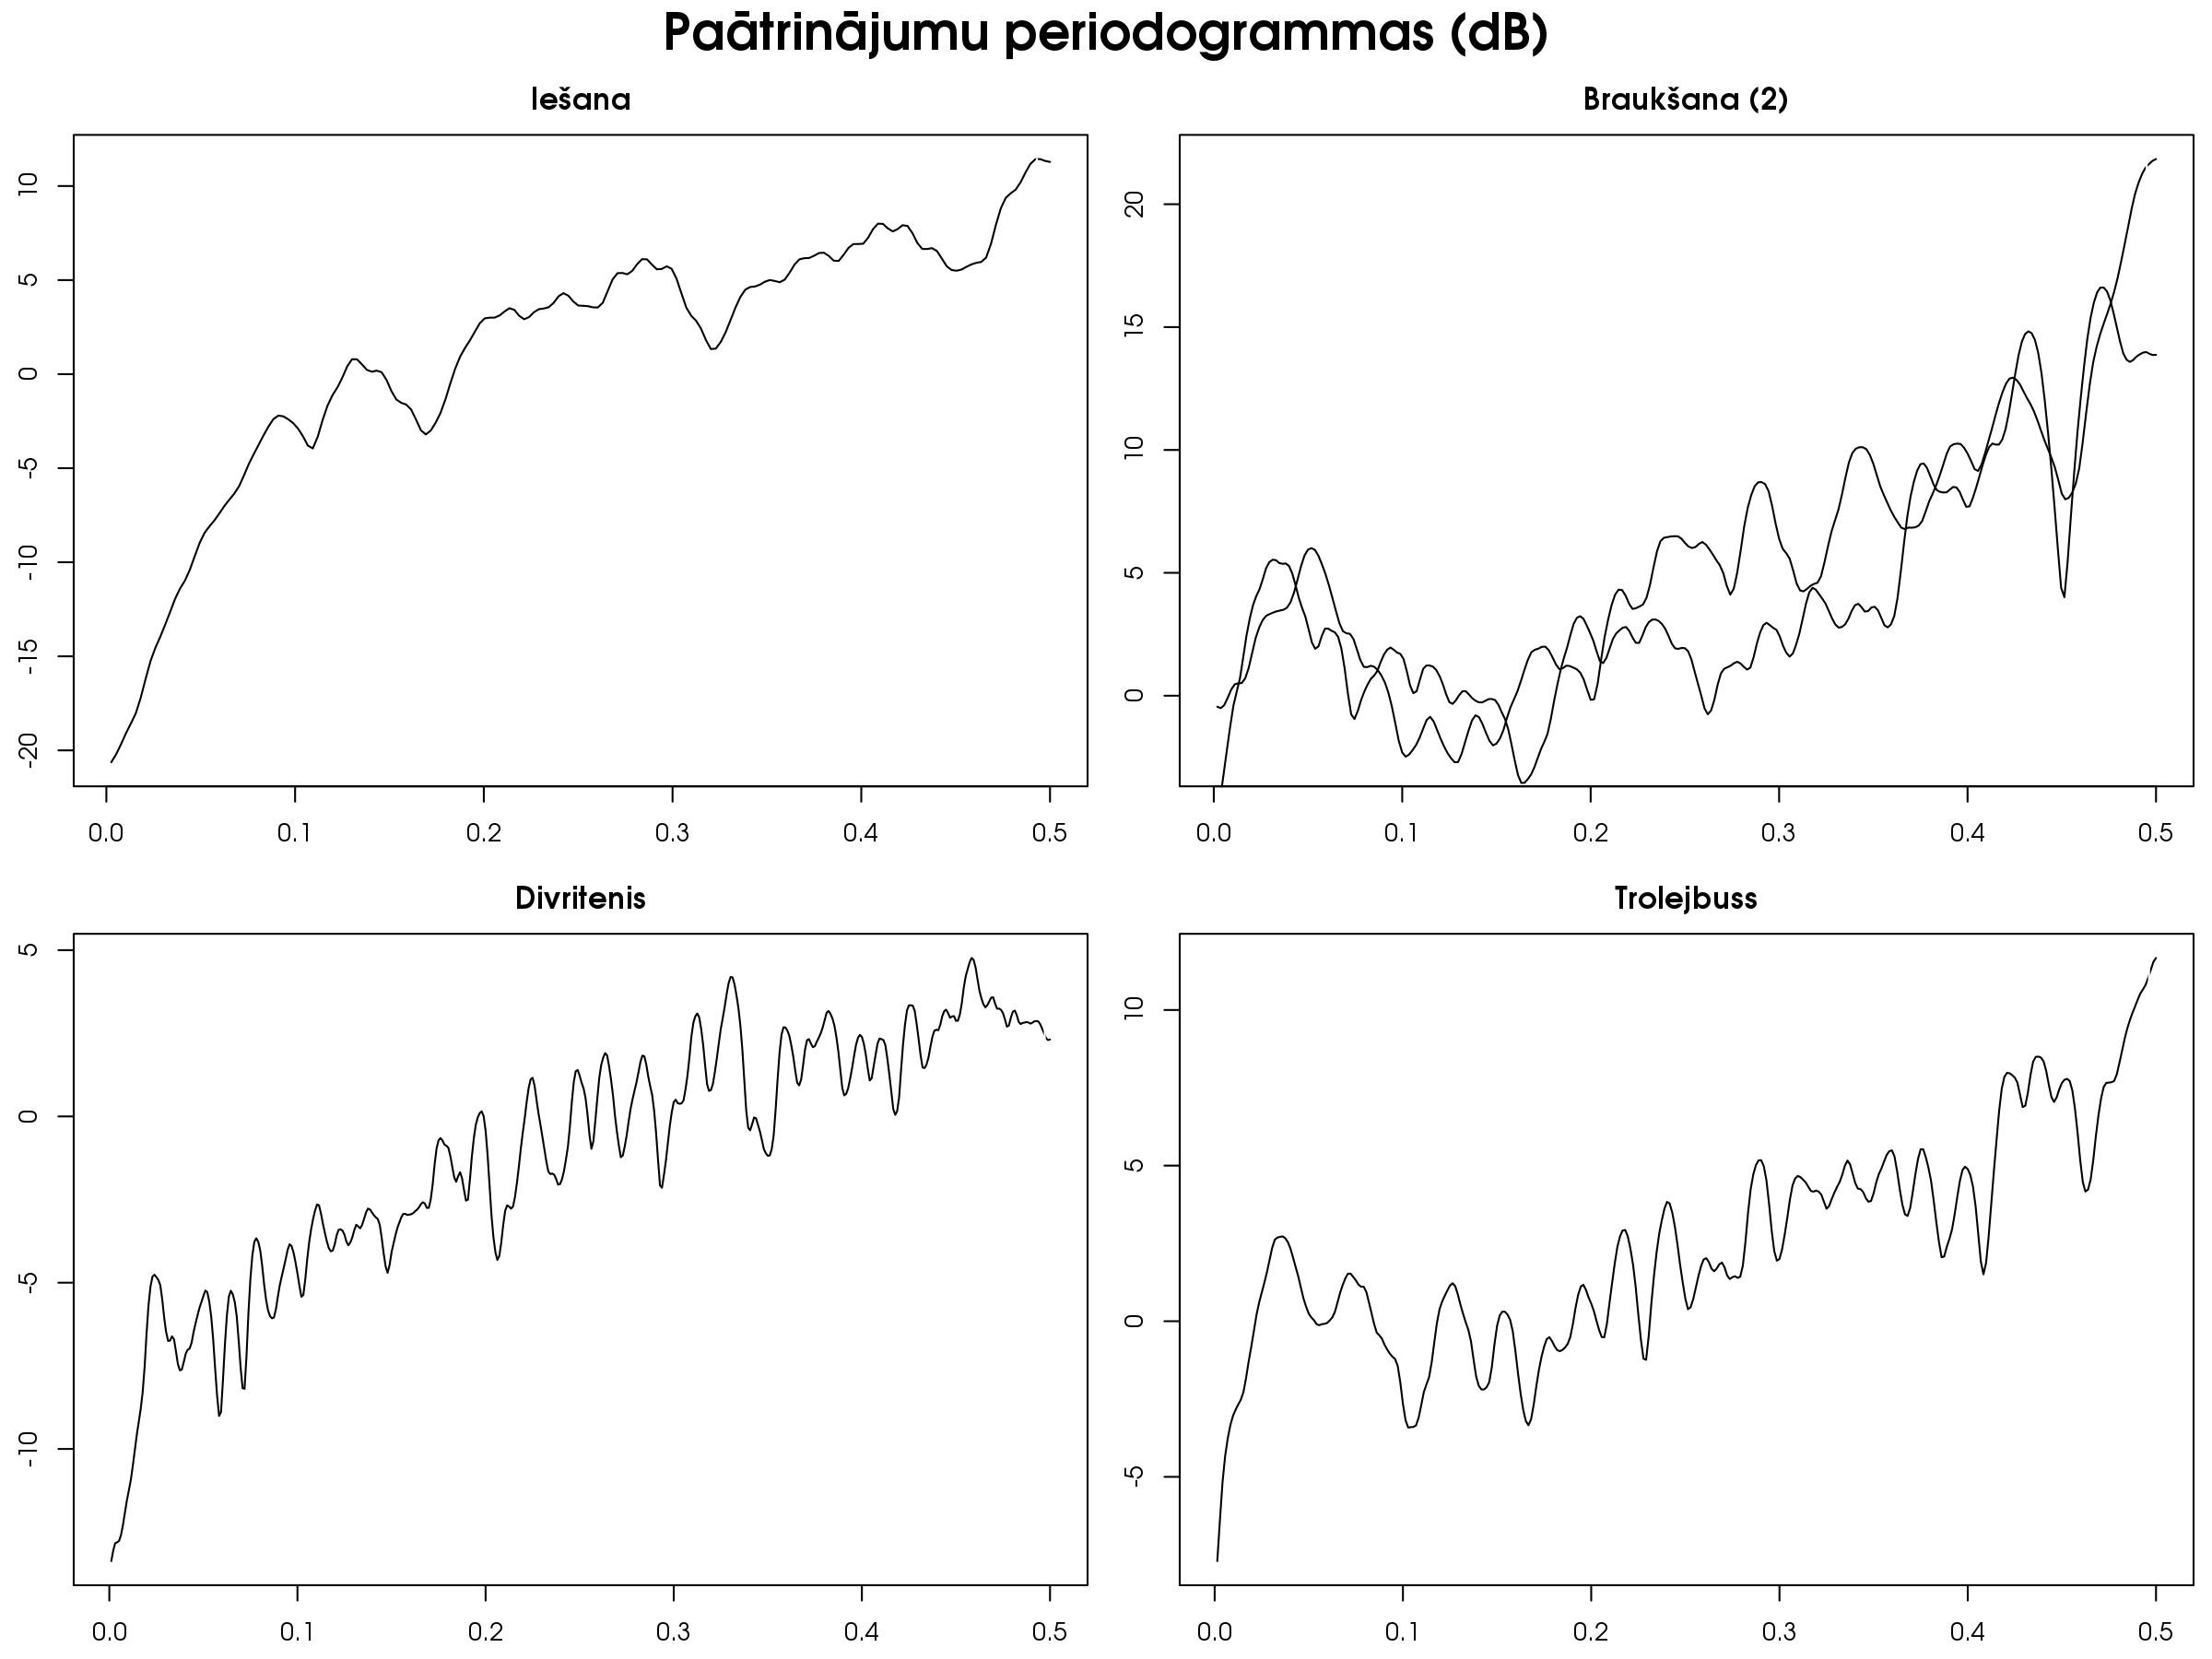
\includegraphics[scale=0.5]{img/periodograms}
  \caption{Dažādu transportu pārvietošanās paātrinājumu periodogrammas}
  \label{fig:periodograms}
\end{figure}

Pēc periodogrammām redzams, ka visus četrus transporta veidus var viegli izšķirt. Tas liek domāt,
ka nogludinātās periodogrammas var lietot kā ieeju klasterizācijas algoritmam.

Segmentu klasterizācijai tiek izmantota \emph{R} ~\cite{Rcore} implementācija \emph{K-means} 
algoritmam, jo:
\begin{itemize}
\item tas ir ātrs;
\item tas garantēti konverģē.
\end{itemize}

Algoritmam ieejā nepieciešami vienādas dimensionalitātes paraugi, taču periodogrammas ir atšķirīgu
garumu. Iespējas ir 
\begin{itemize}
\item izvēlēties dimensiju skaitu, kas vienāds ar garāko paraugu un interpolēt vērtības 
  vajadzīgajām frekvencēm paraugiem ar mazāku dimensionalitāti;
\item pirms veikt Furjē transformāciju, pagarināt paraugu ar $0$ līdz nepieciešamajam garumam.
\end{itemize}

Abas alternatīvas sniedz praktiski identisku gala rezultātu. Tā kā izvēlētā FFT
implementācija ~\cite{commons_math} jau pieprasa, lai parauga garums būtu $2$ pakāpe, 
izvēlēta otrā alternatīva un visi paraugi pirms transformācijas tika pagarināti līdz mazākajai
nepieciešamajai $2$ pakāpei, kas iekļautu visus iegūtos segmentus, dotajā datu 
kopā -- $2^{12} = 2048$.

Pirms klasterizācijas tika atmesti segmenti, kuros sākotnēji bija mazāk nekā $60$ datu punktu (t.i.,
laikā īsāki par $1$ minūti), uzskatot, ka tie satur pārāk maz informācijas un ir segmentācijas
algoritma anomālijas. Periodogrammas tika izteiktas decibelu skalā, lai palielinātu signāla / 
trokšņa attiecību.

Klasteru skaita izvēlei populāra ir t.s. ``elkoņa metode'', saskaņā ar kuru klasteru skaitu $k$
izvēlas pēc attiecīgā klasteru skaita izskaidrotās dispersijas. $k$ izvēlas tādu, ka, palielinot
$k$ par $1$, izskaidrotās dispersijas apjoms manāmi nepalielinās.

Klasteru skaita izskaidrotā dispersijas grafiks redzams attēlā \ref{fig:kmeans_elbow}. Grafikā 
redzams, ka piemērots $k$ ir $6$ vai $7$.

\begin{figure}
  \centering
  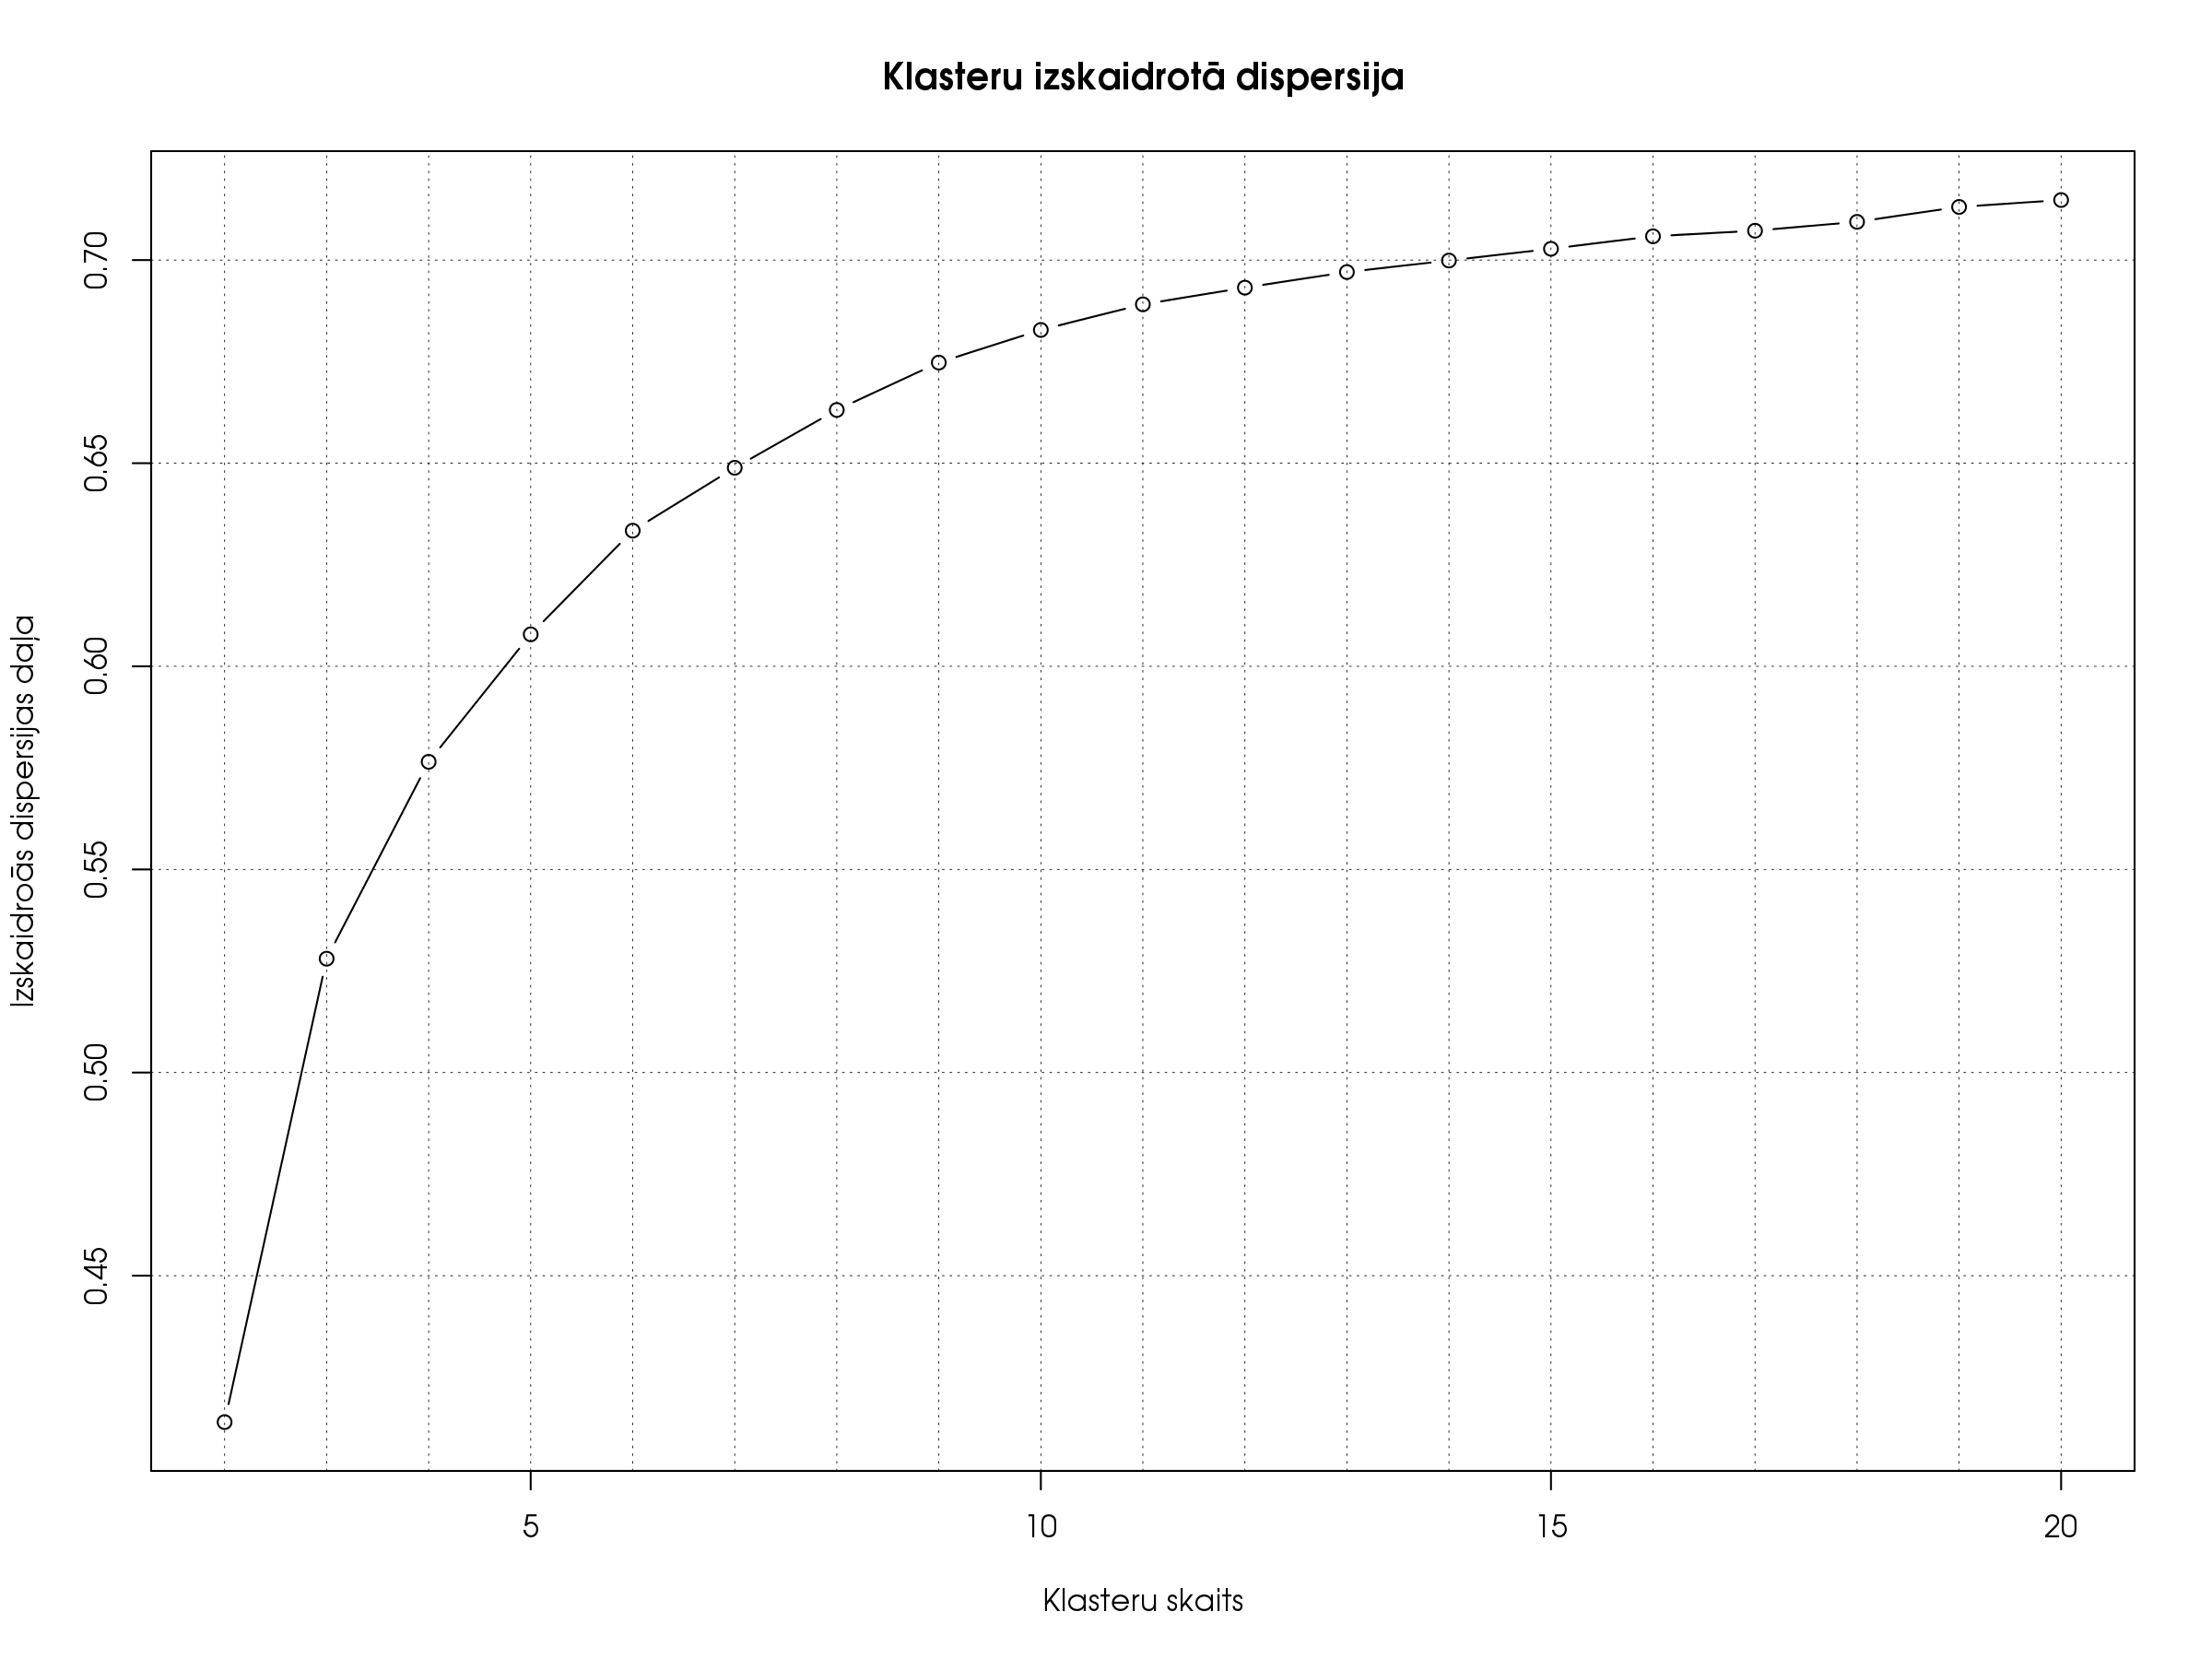
\includegraphics[scale=0.45]{img/kmeans_elbow}
  \caption{Klasteru skaita $k$ izskaidrotā dispersija}
  \label{fig:kmeans_elbow}
\end{figure}

\chapter{Rezultāti}
Izvēloties klasterizēt GPS ceļu segmentus $6$ klasteros redzami labi rezultāti. Attēlā 
\ref{fig:clustered_trails} redzams sagrupēto segmentu grafisks attēlojums. Gaišākie, 
spilgti zilie ceļi aptuveni atbilst maršrutiem, kas datos ir mēroti ar divriteni, violetie -- 
maršrutiem, kas ieti ar kājām, tumši zilie -- ikdienā lietotajiem trolejbusa maršrutiem un liela daļa
sarkano ceļu -- maršrutiem, kas veikti pārvietojoties ar automašīnu.

\begin{figure}
  \centering
  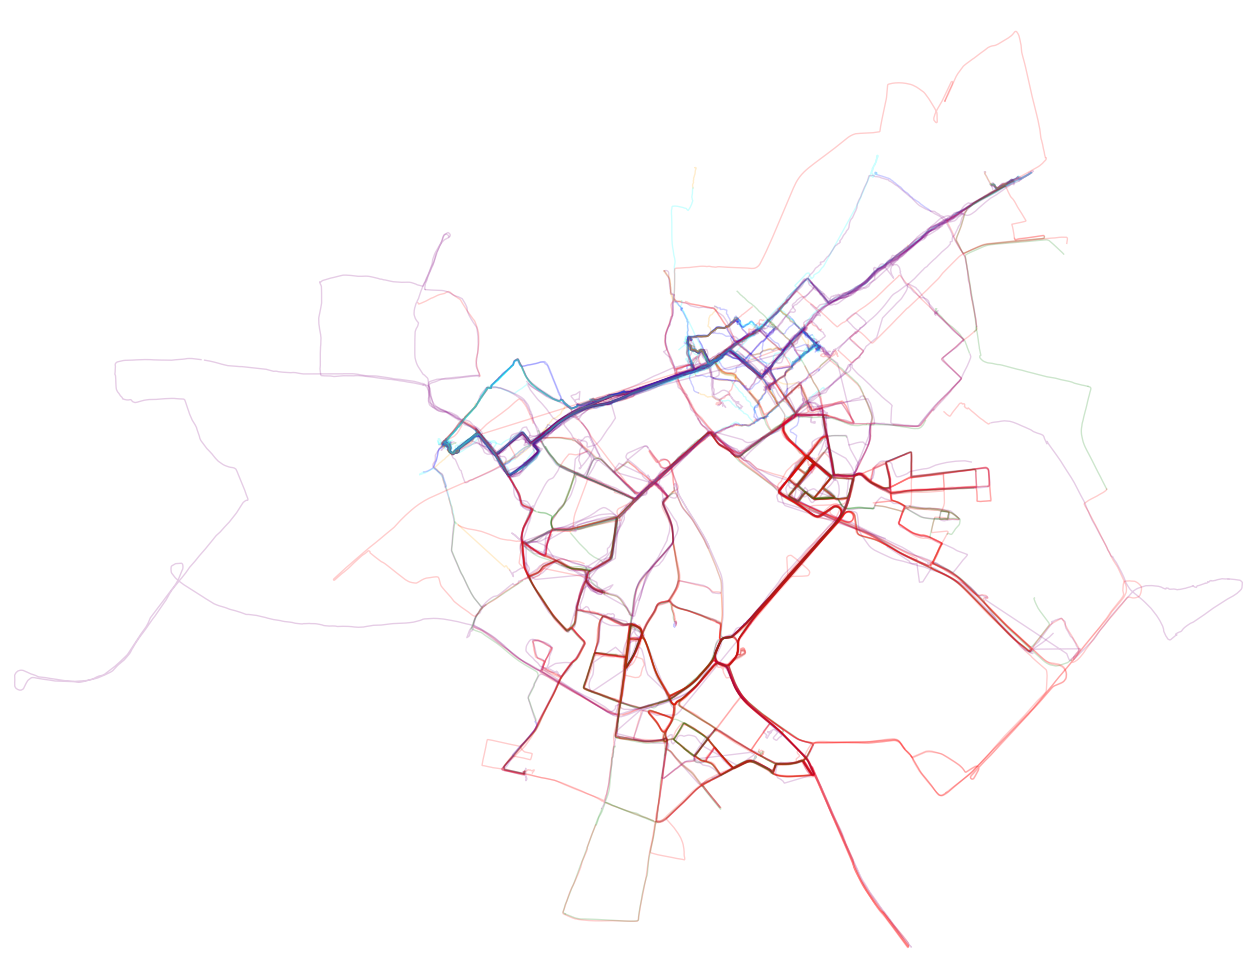
\includegraphics[scale=0.45]{img/clustered_trails}
  \caption{Klasterizēto GPS segmentu projekcija}
  \label{fig:clustered_trails}
\end{figure}

Līdzīgi rezultāti ir arī izvēloties grupēt datus $7$ klasteros.

\section{Kļūdas}
Iegūtajos klasteros ir acīmredzamas kļūdas, piemēram, kreisajā pusē redzamais violetais loks, kaut
gan pārējie violetie ceļa posmi šķietami atbilst ar kājām mērotiem maršrutiem. Konkrētais gadījums
šķietami skaidrojams ar to, ka tas ir ceļš uz lidostu un veikts ārpus pilsētas, līdz ar ko
paātrinājums bijis salīdzinoši konstants. Iespējams šī kļūda tiktu labota, ja par papildus pazīmi
tiktu izvēlēts arī ātrums.

Šī pati kļūda norāda uz vēl vienu apstākli -- ievāktā datu kopa, lai arī sākotnēji šķietami 
vispusīga, ir ar vairākiem trūkumiem. Dati ievākti tikai pilsētā, tajos nav, piemēram, pārvietošanās
pa lielceļiem lielākos ātrumos ar jebkuru transporta līdzekli.

Rezultātos redzama arī viena transporta veida šķelšanās divos klasteros. Ceļi, kas iezīmēti zaļā
krāsā, ir pārvietošanās ar auto, taču tādi ir arī lielākā daļa sarkano. Ticami, ka arī šo
problēmu iespējams atrisināt ar papildus pazīmju ieviešanu.

Iespējams, daļa no klasterizācijas kļūdām skaidrojamas arī ar algoritma pirmā posma kļūdām. 
Pirmajā posmā lietotā algoritma precizitāte ir ap $40\%$. Tas mēdz ieviest dažas tipiskas anomālijas
segmentējot ceļus, piemēram, nošķelt staigāšanas segmentu pa vidu garākam braukšanas segmentam, kaut
gan staigāšana tur nav bijusi. Tam var būt vairākas negatīvas ietekmes:
\begin{itemize}
\item kopējā ne-staigāšanas segmenta garuma samazināšanās. Ekstrēmākos gadījumos, iespējams pat zem
  $60$ s sliekšņa, bet pat ja sašķelts tiek krietni garāks segments -- var gadīties, ka pazīmes
  starp šiem posmiem atšķiras pietiekoši, lai tos sagrupētu dažādās grupās, kaut arī pēc
  abu posmu pazīmju vidējās vērtības posms kopumā pieder kādai citai grupai.
\item vairāki segmenti tiek klasificēti atsevišķi, kaut arī tie ir viens. Tā rezultātā segmenti, kas
  patiesībā ir viens segments var tikt kļūdaini sadalīti vairākās grupās.
\end{itemize}

Ir arī redzamas vietas, kur pirmā posma algoritms konsistenti pieļauj kļūdas lielā daļā datu
paraugu, pārsvarā klasificējot ne-staigāšanas posmus kā staigāšanas. Izteiktākais piemērs ir 
saistīts ar sabiedrisko transportu. Ja tas garāku posmu veic ar zemu ātrumu un paātrinājumu,
algoritms nolemj, ka tas ir staigāšanas posms. Piemērs attēlā \ref{fig:wrong_segmentation} ir viena
no tipiskām kļūdu vietām. Parasti šie kļūdainie segmenti ir īsi, un tos varētu likvidēt ieviešot
pirmā posma algoritmā kādu heiristiku.

% plot(mapproject(andrejsalaSegments$lon, andrejsalaSegments$lat), col=c("green", "red")[andrejsalaSegments$transportMode + 1], type="p", cex=1, xlim=c(-.0003, 0), ylim=c(1.2147, 1.2150), xaxt="n", yaxt="n", main="Nepareizas klasifikācijas piemērs", xlab="", ylab="", pch=c("X", "O")[andrejsalaSegments$transportMode + 1])
% legend(-0.0003, 1.21475, c("Staigāšana", "Nestaigāšana"), col=c("green", "red"), pch=c("X", "O"))
\begin{figure}
  \centering
  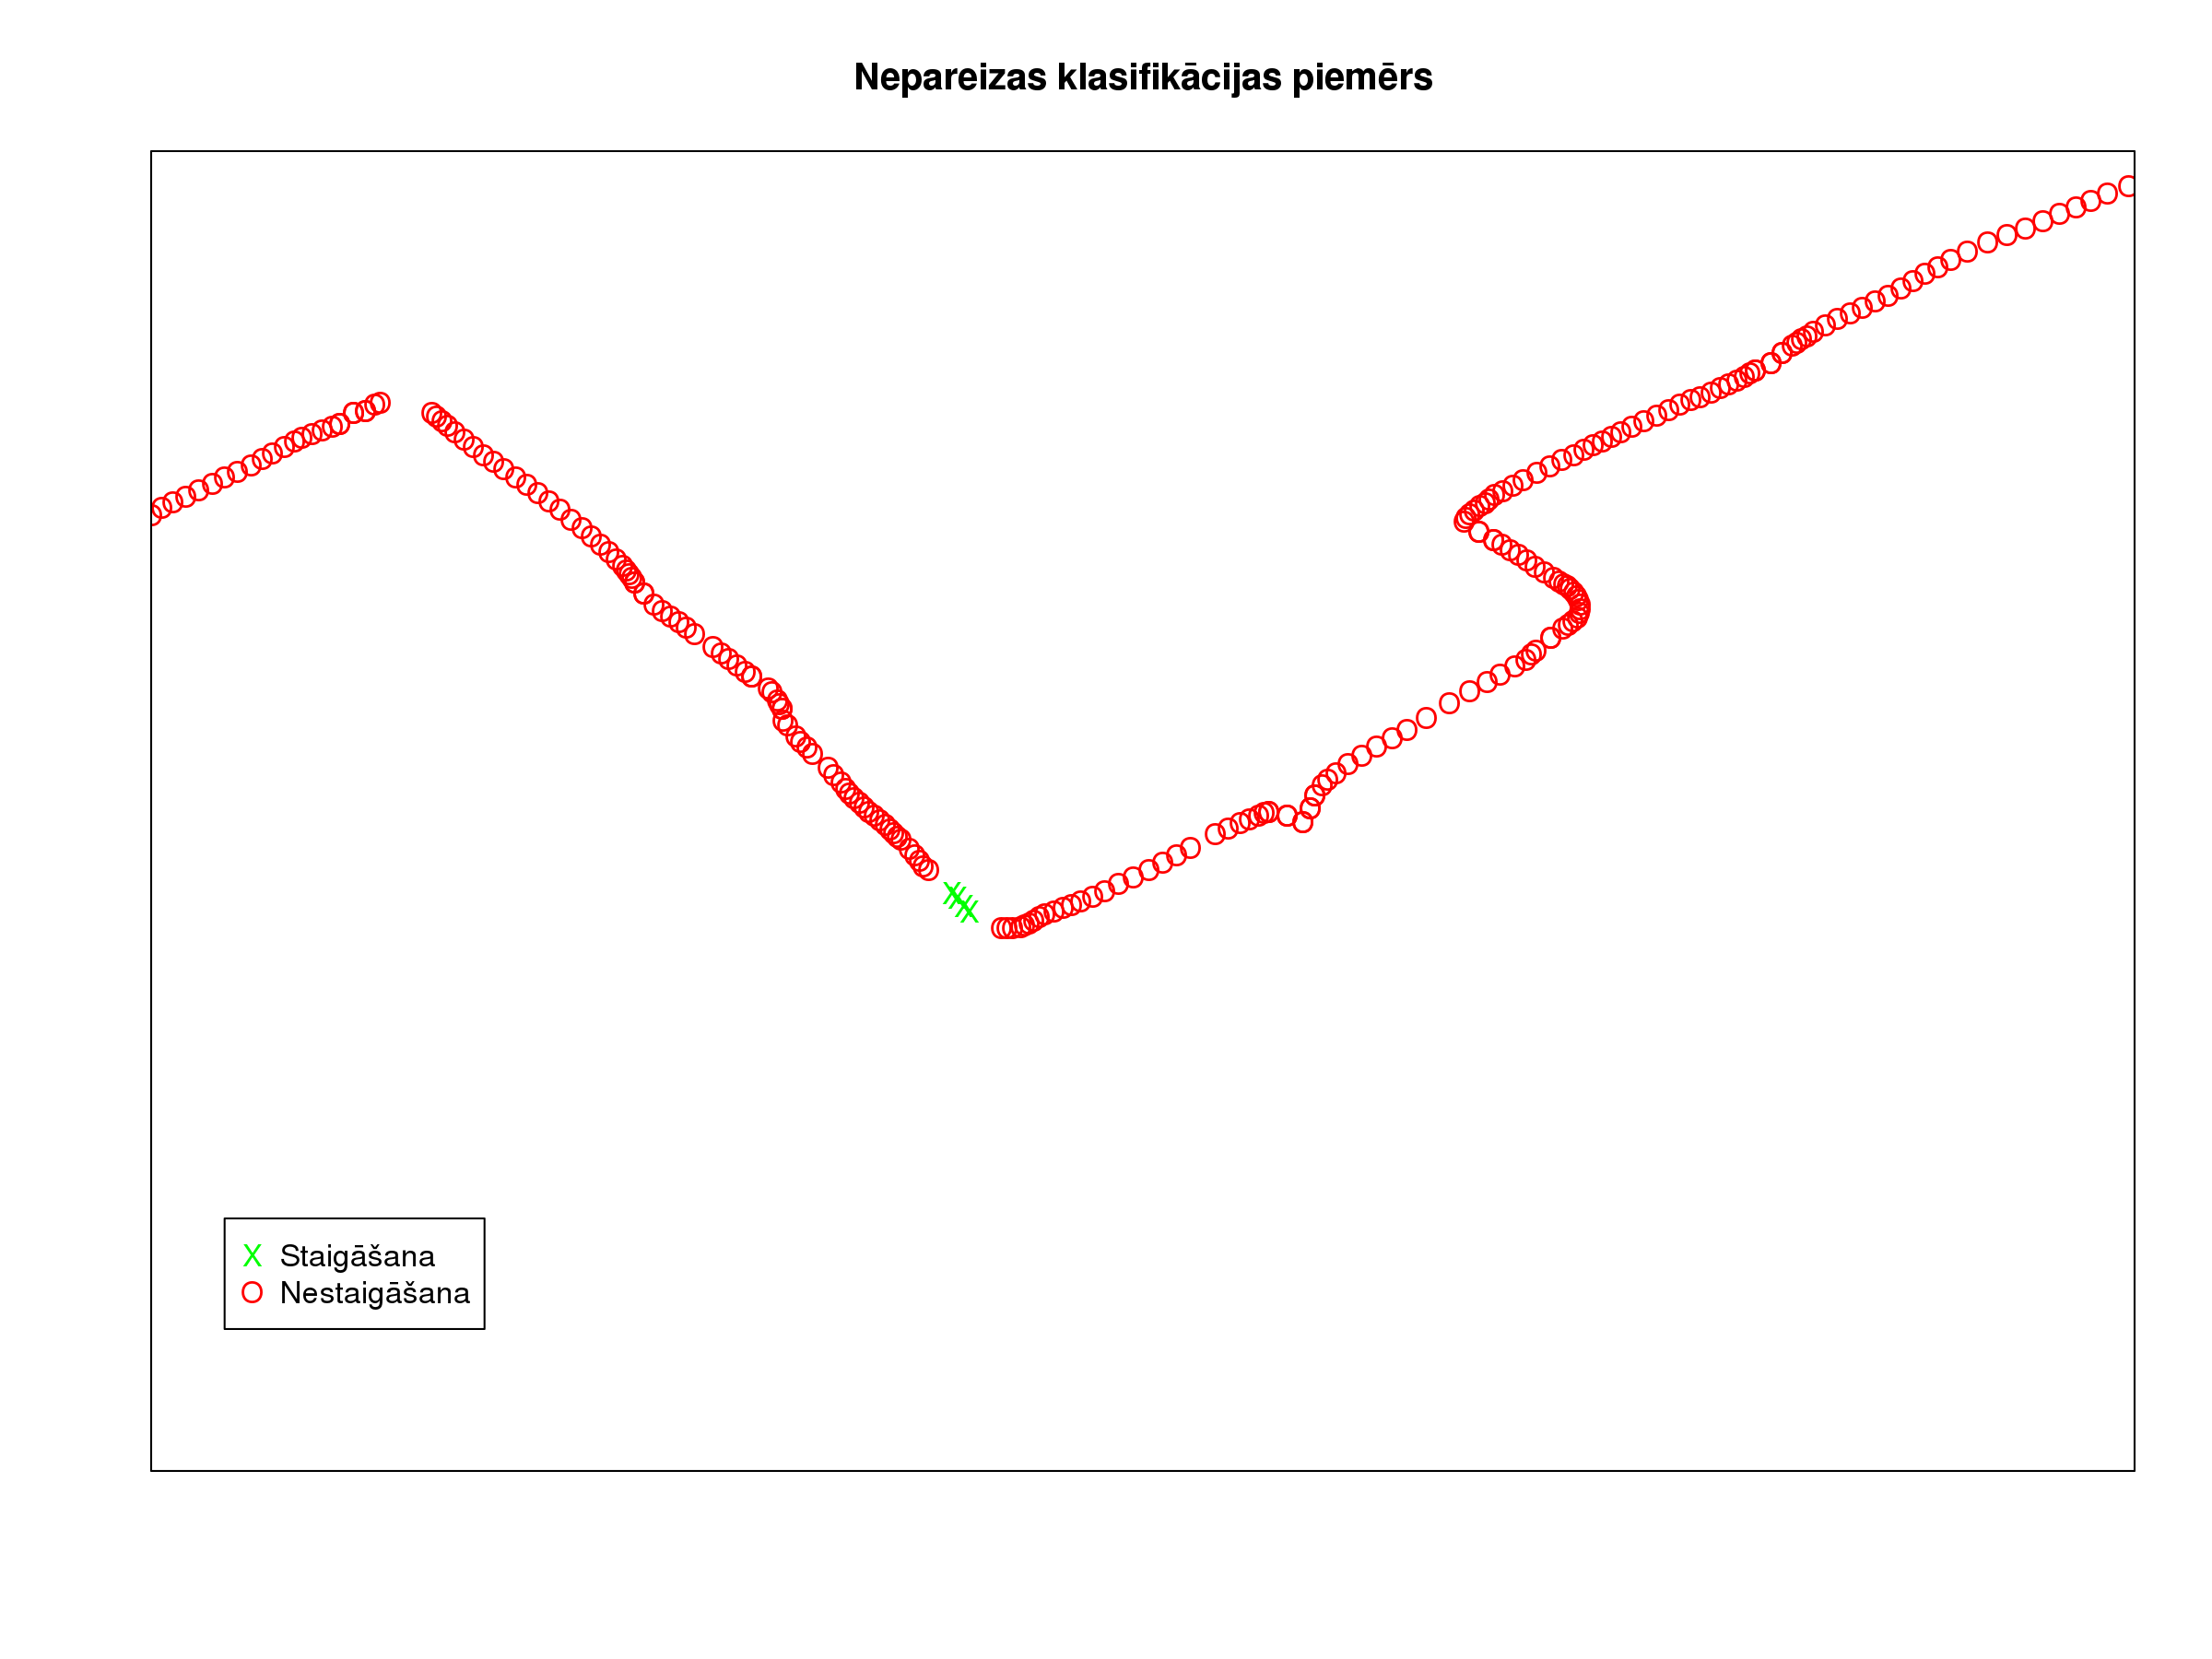
\includegraphics[scale=0.45]{img/wrong_segmentation}
  \caption{Ceļa segmentācijas kļūdas piemērs}
  \label{fig:wrong_segmentation}
\end{figure}

\section{Virzieni tālākai izpētei}
Ir saprātīgi pieņemt, ka algoritma precizitāti varētu ievērojami uzlabot pievienojot papildus
pazīmes, sākot ar ātrumu, bet arī virziena maiņas biežumu un lielumu, apstāšanās biežumu u. tml.

Nepieciešams papildināt un padarīt vispārīgāku ievākto datu kopu. Darba izstrādes gaitā atklātās
nepilnības datos novērst nav grūti, bet ir salīdzinoši laikietilpīgi. Taču bez vispusīgākiem
datiem pastāv risks ka tālāka izpēte būtu tendencioza, ar noslieci uz pilsētas apstākļiem, kas
pats par sevi nav slikti, bet arī nav šī darba mērķis.

Nepieciešams papildināt datus ar citu cilvēku GPS ierakstiem. Pašreizējā datu kopā ir tikai darba
autora ierakstītie GPS ceļi. Katram cilvēkam, iespējams, ir individuāli braukšanas ieradumi, kas
arī varētu ieviest datos liekas tendences.

Noderīgi būtu arī ievākt iezīmētus datus, lai varētu empīriski noteikt klasterizācijas metodes
precizitāti un jutību un salīdzināt to ar uzraudzītās mašīnmācīšanās metodēm.

\chapter{Secinājumi}
Augstā frekvencē ierakstītus GPS datu ceļus ir iespējams veiksmīgi dalīt segmentos un klasterizēt
pēc izmantotā transporta veida. Kaut arī rezultātos ir kļūdas, sasniegta pietiekoši augsta
precizitāte, lai būtu pamats domāt, ka to var tālāk uzlabot strādājot pie abām algoritma
daļām. 

Ir eksperimentāli pierādīts, ka pilsētas apstākļos ievāktus reālus GPS datus ir iespējams
klasterizēt tikai pēc pazīmēm, kas atvasinātas no to paātrinājuma, kas norāda uz to, ka paātrinājums
ir vērtīga pazīme, ko ņemt vērā turpmākajā algoritma izstrādē.

Ņemot vērā darba rezultātus, hipotēzi, ka ierakstītus GPS ceļus iespējams segmentēt un klasterizēt
pēc transporta veidiem var uzskatīt par apstiprinātu.

Izstrādātajā algoritmā klasterizācija veikta izmantojot tikai no paātrinājuma atvasinātas pazīmes,
kā rezultātā atklātas nepilnības ievāktajos datos, bet kuras iespējams risināt ievācot papildu
datus un dažādojot datu ievākšanas vietas un veidus.

\literatura{es09260}

\end{document}
